%!TEX root = ../thesis.tex
\chapter{Isogeometric enhanced SBFEM in 2D}
\label{Iso_sec:main}
\section{Introduction}
\paragraph{}
The main objective of this chapter is to combine the concept of isogeometric analysis and the SBFEM.
Non-uniform rational B-splines (NURBS) basis functions are employed to approximate the unknown fields in the circumferential direction.
This provides a seamless integration with the CAD model.
The method is further extended to problems with singularities within the framework of linear elastic fracture mechanics and to dynamic analysis.
The proposed method enhances the conventional IGA and the salient features of the method are:
    \begin{itemize}
        \item No tensor-product patches as only the boundary information is required for the stress analysis
        \item Feasible to have a n-sided polygonal domain of mixed type/order of the element on the edges, 
                which leads to high flexibility in meshing and mesh transition
        \item Model strain/stress singularities without enrichment
        \item No internal mesh when studying the dynamic response at high frequencies
    \end{itemize}


This chapter organized as follows.
Section.~\ref{iso_section:formulation} provides an overview of the SBFEM and important equations pertaining to linear elasticity,
followed by extending the formulation to linear elastic fracture mechanics in Section~\ref{iso_section:fracture}.
After that, methods that perform the interpolation of surface traction and displacement will be presented in Section~\ref{iso_section:surface_traction} and Section~\ref{iso_section:interpolation}.
Numerical integration with NURBS will be mentioned in Section~\ref{iso_section:numerical_integration} before the accuracy and the convergence properties of the proposed techniques being demonstrated with benchmark problems in the context of linear elasticity and linear elastic fracture mechanics in Section~\ref{iso_section:examples}, followed by concluding remarks in the last section.
This chapter is published \citep{NATARAJAN2015733}.
%=================================================================================================================================%
\section{Formulation of the isogeometric SBFEM}
\label{iso_section:formulation}
The nodal coordinates on the boundary are denoted as $\mathbf{x}_b$. As in a standard 1D iso-parametric finite element, the geometry of the element described by the coordinates $\mathbf{x}_b(\eta)$ as shown in Fig.~\ref{lr_fig:sbfem_intro}, is expressed as
\begin{equation}
    \mathbf{x}_b(\eta) = \mathbf{N}(\eta) \mathbf{x}_b
    \label{lr_eq:sbfem_boundary_interpolate}
\end{equation}
%
where $\mathbf{N}(\eta)$ is the shape function matrix.
Without loss of generality, the origin of the Cartesian coordinate system is chosen at the scaling center.
The geometry of the subdomain, described by $x$, is formed by scaling the boundary (Eq.~\ref{lr_eq:sbfem_boundary_interpolate})
\begin{equation}
    \mathbf{x} = \xi \mathbf{x}_b (\eta)
    \label{lr_eq:sbfem_scaling}
\end{equation}
%
where $\xi$ is the normalized radial coordinate running from the scaling center towards the boundary, with $\xi=0$ at the scaling center and $\xi=1$ on the boundary.
The coordinates $\xi$ and $\eta$ are the so-called scaled boundary coordinates.
They are related to the polar coordinates $r$ and $\theta$.
The transformation is expressed as
\begin{equation}
\begin{aligned}
    r(\xi,\eta) &= \xi r_b(\eta)     \\
    \theta(\eta) &= \arctan \frac{y(\eta)}{x(\eta)}
    \label{lr_eq:sbfem_transform}
\end{aligned}
\end{equation}
%
where $r_b$ is the distance from the scaling center to a point on the boundary.
The transformation between the Cartesian coordinates and the scaled boundary coordinates is similar to the coordinate transformation in the constructing iso-parametric finite elements.
The scaling center must be placed at the position so that all boundary of the domain is visible from the point.
This limitation can be easily solved by using a mesh generation algorithm described in Sec.~\ref{qdt_sec:main}.

The displacement at any point are approximated by
\begin{equation}
    \mathbf{u}(\xi,\eta) = \mathbf{N}(\eta) \mathbf{u}(\xi)
    \label{lr_eq:sbfem_disp_interpolation}
\end{equation}
%
where $\mathbf{N}(\eta)$ are the shape functions of elements on the boundary and $\mathbf{u(\xi)}$ is the displacement along the radial lines, represented by a set of N analytical functions.
By substituting Eq.~\ref{lr_eq:sbfem_disp_interpolation} into the definition of strain-displacement relations, the strain $\epsilon(\xi,\eta)$ are expressed as
\begin{equation}
    \epsilon(\xi,\eta) = \mathbf{Lu}(\xi,\eta)
    \label{lr_eq:sbfem_strain_disp_relation}
\end{equation}
%
where $\mathbf{L}$ is a linear operator matrix formulated in the scaled boundary coordinates
\begin{equation}
    \mathbf{L} =    \mathbf{b}_1(\eta) \frac{\partial}{\partial \xi} +
                    \frac{1}{\xi} \mathbf{b}_2(\eta)
    \label{lr_eq:sbfem_l_operator}
\end{equation}
%
and
\begin{equation}
    \begin{aligned}
    \mathbf{b}_1(\eta) & = \frac{1}{|J|}
            \begin{bmatrix}
                y_b(\eta),_{\eta}   &   0   \\
                0   &   -x_b(\eta),_{\eta}  \\
                -x_b(\eta),_{\eta} & y_b(\eta),_{\eta}
            \end{bmatrix} \\
    \mathbf{b}_2(\eta) & = \frac{1}{|J|}
            \begin{bmatrix}
                -y_b    &   0   \\
                0       &   x_b \\
                x_b     &   y_b
            \end{bmatrix}
    \end{aligned}
    \label{lr_eq:sbfem_little_b}
\end{equation}
%
The determinant of the Jacobian matrix is
\begin{equation}
    |J| = x_b(\eta)y_b(\eta),_{\eta}
        - y_b(\eta)x_b(\eta),_{\eta}
    \label{lr_eq:sbfem_Jdet}
\end{equation}
%
where $x_b(\eta)$ and $y_b(\eta)$ are given by Eq.~\ref{lr_eq:sbfem_boundary_interpolate}.
The stresses $\sigma(\xi,\eta)$ are given by:
\begin{equation}
    \sigma(\xi,\eta) =  \mathbf{DB}_1(\eta) \mathbf{u}(\xi),_{\xi} +
                        \frac{1}{\xi} \mathbf{DB}_2(\eta) \mathbf{u}(\xi)
    \label{lr_eq:sbfem_stress}
\end{equation}
%
where in the above equation, the definition of strain and the linear operator matrix given by Eq.~\ref{lr_eq:sbfem_strain_disp_relation} and Eq.~\ref{lr_eq:sbfem_l_operator} are used with
\begin{equation}
    \begin{aligned}
        \mathbf{B}_1(\eta) &= \mathbf{b}_1(\eta) \mathbf{N}(\eta)    \\
        \mathbf{B}_2(\eta) &= \mathbf{b}_2(\eta) \mathbf{N}(\eta),_{\eta}
        \label{lr_eq:sbfem_captial_b}
    \end{aligned}
\end{equation}
%
substituting Eq.~\ref{lr_eq:sbfem_strain_disp_relation} and Eq.~\ref{lr_eq:sbfem_stress} in the virtual work statement for elastostatics \citep{Deeks2002} and following the derivation
\begin{equation}
    \begin{aligned}
        \delta \mathbf{u}(\xi)^{T} \left(
            (\mathbf{E}_0 \xi \mathbf{u}(\xi),_{\xi}
            + \mathbf{E}_1^T \mathbf{u}(\xi))|_{\xi=1}
            - \mathbf{F}
        \right) - \\
        \int_0^1 \delta u(\xi)^T\left(
            \mathbf{E}_0 \xi^2 \mathbf{u}(\xi),_{\xi\xi} + (\mathbf{E}_0 + \mathbf{E}_1^T - \mathbf{E}_1) \xi \mathbf{u}(\xi),_{\xi}
            - \mathbf{E}_2 u(\xi)
        \right) d\xi = 0
    \end{aligned}
    \label{lr_eq:sbfem_virtual_work}
\end{equation}
%
where $\mathbf{u}(\xi)$ is the nodal displacement vector and $\mathbf{F}$ is the vector of equivalent boundary nodal forces, given by:
\begin{equation}
    \mathbf{F} = (\mathbf{E}_0 \xi \mathbf{u}(\xi),_{\xi} + \mathbf{E}_1^T \mathbf{u}(\xi))|_{\xi=1}
    \label{lr_eq:sbfem_nodal forces}
\end{equation}
%
By considering the arbitrariness of $\delta \mathbf{u}(\xi)$, the following ODE is obtained:
\begin{equation}
    \mathbf{E}_0 \xi^2 \mathbf{u}(\xi),_{\xi\xi} + (\mathbf{E}_0 + \mathbf{E}_1^T - \mathbf{E}_1)\xi \mathbf{u}(\xi),_{\xi} - \mathbf{E}_2 \mathbf{u}(\xi) = 0
    \label{lr_eq:sbfem_ODE}
\end{equation}
%
where $\mathbf{E}_0$, $\mathbf{E}_1$ and $\mathbf{E}_2$ are known as the coefficient matrices and are given by:
\begin{equation}
    \begin{aligned}
        \mathbf{E}_0 &= \int_\eta \mathbf{B}_1(\eta)^T \mathbf{DB}_1(\eta)|J|d\eta \\
        \mathbf{E}_1 &= \int_\eta \mathbf{B}_2(\eta)^T \mathbf{DB}_1(\eta)|J|d\eta \\
        \mathbf{E}_2 &= \int_\eta \mathbf{B}_2(\eta)^T \mathbf{DB}_2(\eta)|J|d\eta
    \end{aligned}
    \label{lr_eq:sbfem_coe_matrix}
\end{equation}
%
Eq.~\ref{lr_eq:sbfem_ODE} is a homogeneous second-order differential equation.
Its solution is obtained by introducing the variable $\mathbf{\chi}(\xi)$
\begin{equation}
    \mathbf{\chi} = \left\{
        \begin{matrix}
            \mathbf{u}(\xi)  \\
            \mathbf{q}(\xi)
        \end{matrix}
    \right\}
    \label{lr_eq:sbfem_ODE_soltion}
\end{equation}
%
where $\mathbf{q}(\xi)$ is the internal force vector
\begin{equation}
    \mathbf{q}(\xi) =   \mathbf{E}_0 \xi \mathbf{u}(\xi),_{\xi} +
                        \mathbf{E}_1^T \mathbf{u}(\xi)
    \label{lr_eq:sbfem_internal_force}
\end{equation}
%
The boundary nodal forces are related to the displacement functions by:
\begin{equation}
    \mathbf{F} = \mathbf{q}(\xi=1) = (\mathbf{E}_0\xi \mathbf{u}(\xi),_{\xi} + \mathbf{E}_1^T\mathbf{u}(\xi))|_{\xi=1}
    \label{lr_eq:sbfem_boundary_nodal_force}
\end{equation}
%
This allows Eq.~\ref{lr_eq:sbfem_ODE} to be transformed into a first order ordinary differential equation with twice the number of unknowns as:
\begin{equation}
    \xi \mathbf{\chi}(\xi),_{\xi} = -\mathbf{Z} \mathbf{\chi}(\xi)
    \label{lr_eq:sbfem_1stODE}
\end{equation}
%
where $\mathbf{Z}$ is a Hamiltonian matrix
\begin{equation}
    \mathbf{Z} = \begin{bmatrix}
        \mathbf{E}_0^{-1} \mathbf{E}_1^T    &  -\mathbf{E}_0^{-1}   \\
        \mathbf{E}_1 \mathbf{E}_0^{-1} \mathbf{E}_1^T - \mathbf{E}_2    &   -\mathbf{E}_1 \mathbf{E}_0^{-1}
    \end{bmatrix}
    \label{lr_eq:sbfem_zmatrix}
\end{equation}
%
An eigenvalue decomposition of $\mathbf{Z}$ is performed and it yields:
\begin{equation}
    \mathbf{Z} \begin{bmatrix}
        \mathbf{\Phi}_u \\
        \mathbf{\Phi}_q
    \end{bmatrix} = \begin{bmatrix}
        \mathbf{\Phi}_u  \\
        \mathbf{\Phi}_q
    \end{bmatrix} \mathbf{\Lambda}_n
    \label{lr_eq:sbfem_eigen_decomp}
\end{equation}
%
In Eq.~\ref{lr_eq:sbfem_eigen_decomp}, $\mathbf{\Lambda}_n$ $=$ diag$(\lambda_1$, $\lambda_2$, $\dots$, $\lambda_n)$ contains only the eigenvalues with negative real part.
$\mathbf{\Phi}_u$ and $\mathbf{\Phi}_q$ are the subsets of the eigenvectors corresponding to $\mathbf{Lambda}_n$.
They represent the modal displacements and forces, respectively.
The general solution of Eq.~\ref{lr_eq:sbfem_1stODE} is given by:
\begin{align}
    \mathbf{u}(\xi) &= \mathbf{\Phi}_u \xi^{-\mathbf{\Lambda_n}} \mathbf{c}
    \label{lr_eq:sbfem_general_sol_disp} \\
    \mathbf{q}(\xi) &= \mathbf{\Phi}_q \xi^{-\mathbf{\Lambda_n}} \mathbf{c}
    \label{lr_eq:sbfem_general_sol_str}
\end{align}
%
where $\mathbf{c}$ are integration constants that are obtained from the nodal displacements $\mathbf{u}_b = \mathbf{u}(\xi=1)$ as:
\begin{equation}
    \mathbf{c} = \mathbf{\Phi}_u^{-1} \mathbf{u}_b
    \label{lr_eq:sbfem_int_constant}
\end{equation}
%
The complete displacement field of a point defined by the sector covered by a line element on the boundary is obtained by substituting Eq.~\ref{lr_eq:sbfem_general_sol_str} into Eq.~\ref{lr_eq:sbfem_disp_interpolation} resulting in:
\begin{equation}
    \mathbf{u}(\xi,\eta) = \mathbf{R}(\eta) \mathbf{\Phi}_u \xi ^{-\mathbf{\Lambda}_n} c
    \label{lr_eq:sbfem_displacement_field}
\end{equation}
%
Taking the derivative of $\mathbf{u}(\xi)$ with respect to $\xi$ and substituting into Eq.~\ref{lr_eq:sbfem_stress} the stress field $\sigma(\xi,\eta)$ can be expressed as:
\begin{equation}
    \sigma(\xi,\eta) = \mathbf{\Psi}_\alpha (\eta) \xi^{-\mathbf\Lambda}_n - \mathbf{I} \mathbf{c}
    \label{lr_eq:sbfem_stress_field}
\end{equation}

where the stress mode $\mathbf{\Psi}_\sigma(\eta)$ is defined as:
\begin{equation}
    \mathbf{\Psi}_\alpha(\eta) =    \mathbf{D}(
                                       -\mathbf{B}_1(\eta) \mathbf{\Phi}_u \mathbf{\Lambda}_n +
                                        \mathbf{B}_2(\eta) \mathbf{\Phi}_u
                                    )
    \label{lr_eq:sbfem_stress_mode}
\end{equation}

The stiffness matrix of an element is obtained by first substituting Eq.~\ref{lr_eq:sbfem_int_constant} into Eq.~\ref{lr_eq:sbfem_general_sol_str} at $\xi=1$.
This results in:
\begin{equation}
    \mathbf{F} = \mathbf{\Phi}_q \mathbf{\Phi}_u^{-1} \mathbf{u}_b
    \label{lr_eq:sbfem_kmat_previous}
\end{equation}

From Eq.~\ref{lr_eq:sbfem_kmat_previous}, the stiffness matrix $\mathbf{K}$ can be identified to be given by the expression
\begin{equation}
    \mathbf{K} = \mathbf{\Phi}_q \mathbf{\Phi}_u^{-1}
    \label{lr_eq:sbfem_kmat}
\end{equation}

The SBFEM has recently been extended to dynamic analysis in bounded domains \citep{Song2009}.
Assuming time-harmonic behavior, the scaled boundary equation in displacement is extended as:
\begin{equation}
    \mathbf{E}_0 \xi^2 \mathbf{u}(\xi),_{\xi\xi} +
    (\mathbf{E}_0 + \mathbf{E}_1^T - \mathbf{E}_1)\xi \mathbf{u}(\xi),_{\xi} -
    \mathbf{E}_2 \mathbf{u}(\xi) + \omega^2 \mathbf{M}_0 \xi^2 \mathbf{u}(\xi) = 0
    \label{lr_eq:sbfem_dynamic}
\end{equation}

Where $\mathbf{M}_0$ is a coefficient matrix defined as
\begin{equation}
    \mathbf{M}_0 = \int_\eta \mathbf{N}^T \rho \mathbf{N}|J| d\eta
    \label{lr_eq:sbfem_dynamic_mass}
\end{equation}

Using Eq.~\ref{lr_eq:sbfem_internal_force} and Eq.~\ref{lr_eq:sbfem_boundary_nodal_force}, Eq.~\ref{lr_eq:sbfem_dynamic_mass} can be transformed into an equivalent first-order non-linear differential equation in dynamic stiffness $\mathbf{S}(\omega)$,
\begin{equation}
    (\mathbf{S}(\omega)-\mathbf{E}_1)\mathbf{E}_0^{-1}
    (\mathbf{S}(\omega)-\mathbf{E}_1^T) - \mathbf{E}_2 +
    \omega \mathbf{S}(\omega),_\omega + \omega^2 \mathbf{M}_0 = 0
    \label{lr_eq:sbfem_dynamic_1stODE}
\end{equation}

The dynamic stiffness matrix $\mathbf{S}(\omega)$ relates the nodal forces to the displacements at the boundary as,
\begin{equation}
    \mathbf{F} = \mathbf{S}(\omega) \mathbf{u}(\xi=1)
    \label{lr_eq:sbfem_dynamic_nodal_force}
\end{equation}

Eq.~\ref{lr_eq:sbfem_dynamic_1stODE} is solved by expanding the dynamic stiffness into a series of continued fractions.
For this purpose, it is expressed as
\begin{equation}
    \mathbf{S}(\omega) = \mathbf{K} - \omega^2 \mathbf{M} + \omega^4 \left[
        \mathbf{R}^{(1)}    
    \right]^{-1}
    \label{lr_eq:sbfem_dynamic_stiffness}
\end{equation}

In Eq.~\ref{lr_eq:sbfem_dynamic_stiffness}, the first two terms represent the low-frequency expansion of the dynamic stiffness, whereas the third term corresponds to the residual of the low-frequency approximation.
Substituting Eq.~\ref{lr_eq:sbfem_dynamic_stiffness} in Eq.~\ref{lr_eq:sbfem_dynamic_1stODE} and equating terms in increasing order of powers of $\omega$ to zero yields equations for $\mathbf{K}$ ,$\mathbf{M}$  and $\mathbf{R}^{(1)}$.
Setting the constant terms equal to zero yields an algebraic Riccati equation for the static stiffness matrix $\mathbf{K}$, which is equivalent to the solution process described earlier.
Setting all terms in $\omega^2$ equal to zero yields a Lyapunov equation for the low-order mass matrix $\mathbf{M}$.
The solution procedure of that Lyapunov equation is described in detail in \citep{Son1997}.
The remaining equation for the residual is solved by expanding  $\mathbf{R}^{(1)}$ as
\begin{equation}
    \mathbf{R}^{(1)} = \mathbf{S}_0^{(1)} - \omega^2 \mathbf{S}_1^{(1)} + \omega^4 [\mathbf{R}^{(2)}]^{-1}
    \label{lr_eq:sbfem_dynamic_R}
\end{equation}

Eq.~\ref{lr_eq:sbfem_dynamic_R} is analogous to the expansion of the dynamic stiffness, Eq.~\ref{lr_eq:sbfem_dynamic_stiffness}, where the coefficients $\mathbf{S}^{(1)}_0$ and $\mathbf{S}^{(1)}_1$ correspond to the `stiffness' and `mass' term of $\mathbf{R}^{(1)}$, respectively.
Equations for $\mathbf{S}^{(1)}_0$ and $\mathbf{S}^{(1)}_1$ are found by substituting Eq.~\ref{lr_eq:sbfem_dynamic_R} into the equation for $\mathbf{R}^{(1)}$.
This procedure is continued until the residual $\mathbf{R}^{M_{cf}+1}$ can be neglected.
The symbol of $M_{cf}$ denotes the order of continued-fraction expansion.
Substituting all terms of the expansion back into Eq.~\ref{lr_eq:sbfem_dynamic_stiffness} yields:
\begin{dmath}
    \mathbf{S}(\omega) =    \mathbf{K} - \omega^2 \mathbf{M} + \omega^4 \left(
                                \mathbf{S}_0^{(1)} - \omega^2 \mathbf{S}^{(1)} + \omega^4 \left(
                                    \mathbf{S}_0^{(2)} - \omega^2 \mathbf{S}^{(2)} + \dots + 
                                    \omega^4 \left(
                                        \mathbf{S}_0^{(M_{cf})} - \omega^2 \mathbf{S}_1^{(M_{cf})}
                                    \right)^{-1}
                                \right)^{-1}
                            \right)^{-1}
\label{lr_eq:sbfem_dynamic_s_full}
\end{dmath}

The coefficients $\mathbf{S}^{(i)}_0$ and $\mathbf{S}^{(i)}_1$ in Eq.~\ref{lr_eq:sbfem_dynamic_s_full} are calculated following a recursive procedure.
A more detailed derivation can be found in \citep{Song2009}.
\subsection{Application of isogeometric SBFEM to linear elastic fracture mechanics}

    \begin{equation}
        \sigma(r,\eta) = \sum_i^n
            c_i r^{-(\lambda_i+1)} \left(
                r_\eta^{\lambda_i+1} (\eta)
                \boldsymbol{\psi}_{\sigma_i}(\eta)
            \right)
        \label{iso_eq:isosbfem_fracture_stress_field}
    \end{equation}

\pagebreak
\section{Surface traction}
\label{iso_section:surface_traction}
\paragraph{}
In structural analysis, it is common to have boundary conditions such as displacement constraints and applied loads.
Due to the property of the NURBS that the control points are not necessarily on the curve, surface tractions can not be applied by the same method used in conventional numerical method like FEM or SBFEM.
A surface traction $\Phi$ can be regarded as a Neumann boundary condition which can be expressed as
    \begin{equation}
        {F}=-\int_{\Gamma}
        [N]
        \Phi_n
        d\Gamma
    \label{iso_eq:neumann_bc}
    \end{equation}
where $[N]$ describe the shape functions and $\Phi_n$ is the surface tractions on the nodes.

\paragraph{}
As mentioned in \hl{Sec.}~\ref{iso_section:numerical_integration}, numerical integration would be preferred over mathematical deduction when the target function is an input.
In the flavour of numerical integration, Eq.~\ref{iso_eq:neumann_bc} can be expressed as followed.
    \begin{equation}
        {F}=-\sum_{i=1}^n
        a_i
        [N(\xi_i)]
        \Phi_n
    \label{iso_eq:neumann_bc_numerical}
    \end{equation}
where $\xi_i$ is the integration point and $a_i$ is the weight,
$n$ is the number of integration points and different quadrature rules require different number of points in order to achieve an optimal accuracy.

\paragraph{}
It can be found that the term $[N(\xi_i)] \Phi_n$ is corresponding to $f(x)$ in Eq.~\ref{iso_eq:numerical_integration}.
In conventional FEM or SBFEM, $\Phi_n$ can be determined as the real values on the nodes because, geometrically speaking, its shape function is interpolated from the given set of points.
In other words, all nodes that determine the shape function in traditional FEM or SBFEM must be on the interpolating function.
However, this is not the case in NURBS curves where it is the control points that play the same role as the nodes in existing shape function.
In NURBS curves, apart from the first and the last points, the control points are not necessarily on the curves as illustrated in Fig.~\ref{lr_fig:nurbs_knotins}.
This prevent\hl{s} us from adopting physical value\hl{s} on the nodes as $\Phi_n$ in Eq.~\ref{iso_eq:neumann_bc_numerical}.
Instead, a set of ``control stress'' $\Phi_c$, the control points of another NURBS curve that represent the surface traction geometrically, need to be determined as 
    \begin{equation}
        \Phi_c = \argmin_{\Phi_c}
            \frac{1}{2}
            \int_{-1}^1
            \|
                \Phi(\xi)-
                    \left[ N(\xi) \right]
                    \Phi_c
            \|^2
            d\xi            
    \label{iso_eq:surface_traction_fitting}
    \end{equation}
%
It means that ``control stress'' $\Phi_c$ describe a minimum mean squared error between surface traction NURBS curve and the real traction $\Phi$.
One of the simplest mathematical method\hl{s} to determine $\Phi_c$ will be the least square method.
Given the fact that the shape functions of this NURBS curve will be the same as that describe the geometry, $\left[ N(\xi) \right]$ can be considered as known.
By selecting $n$ sample points over the domain of the $\Phi$, Eq.~\ref{iso_eq:surface_traction_fitting} can be rewrite as
    \begin{equation}
        \Phi_c = \argmin_{\Phi_c}
            \frac{1}{n}
            \sum_{i=1}^n
            \|
                \Phi(\xi_i)-
                    \left[ N(\xi_i) \right]
                    \Phi_c
            \|^2
    \label{iso_eq:surface_traction_fitting_discrete}
    \end{equation}
Then ``control stress'' $\Phi_c$ can be solved by least square as
    \begin{equation}
        \Phi_c= \left(
            \left[ N(\xi) \right] ^T
            \left[ N(\xi) \right]
        \right)^{-1}
        \left[ N(\xi) \right]^T
        \Phi(\xi)
    \end{equation}
and Eq.~\ref{iso_eq:neumann_bc_numerical} in the case where NURBS is in use can be rewrite as
    \begin{equation}
        {F}=-\sum_{i=1}^n
        a_i
        [N(\xi_i)]
        \Phi_c
    \label{iso_eq:neumann_bc_numerical_NURBS}
    \end{equation}

\subsection{Displacement interpolation}
\paragraph{}
Another difference between it with conventional FEM or SBFEM lies in the post processing.
After solving the partial differential equation numerically, the displacements on the nodes will be one of the output in
    the traditional method.
However, similar to what is discussed in \ref{subsection:surface_traction}, NURBS curves are defined by the control points
    that are not geometrically located on the curves.
As a consequence, not only the input such as surface traction need to be translated into a NURBS-like representation, the
    output such as the displacements will be the dummy values on the control points as well, or ``control displacements''
    $\left\{ u_c \right\}$.
Dislike that in the traditional method, the ``control displacements'' do not have any physical meaning. It can only be used
    to interpolate the real displacements within its span.

\begin{equation}
    \left\{ u \right\}=
    \sum_{i=0}^n
    R(u) \left\{u^{(N)}\right\}
\label{eq:displacement_interpolation}
\end{equation}
\pagebreak
\subsection{Numerical integrations}
\label{subsection:numerical_integration}
\paragraph{}
When computing the integrations in SBFEM % equation
    , numerical integrations tends to be overwhelmingly preferred over mathematical deduction. 
The reason behind lies in the flexibility of the numerical and that deduction of exact integrations scheme 
    to any given shape functions are not feasible. 
Due to the fact that the polynomials are adopted as the shape function, the numerical integrations methods 
    such as Legendre Quadrature or Gauss Quadrature provides possibility for an exact integration. 
An integration quadrature is normally defined as followed:
    \begin{equation}
        \int_{-1}^{1}
        f(x)dx 
        = \sum_{i=1}^n
        a_i f(x_i)
    \label{iso_eq:numerical_integration}
    \end{equation}

\paragraph{}
Any given targeted polynomial function defined on $[-1,1]$ can be explicitly expressed as series.
A set of integration points $\left\{ x_1, x_2, \dots, x_n \right\} \in \left[-1,1\right]$ and the corresponding weight $\left\{ a_1, a_2, 
    \dots, a_n \right\} \in \mathbb{R}$ determined from the integration quadrature can be adopted to perform an exact integration
    on the given function.
\paragraph{}
Although shape functions used in NURBS are not polynomials, they can be separated into several spans where the function is a 
    rational polynomial. 
Based on this property, we are able to apply the numerical integration quadrature on each of these spans and achieve a reasonably 
    accurate result.
In other words, the NURBS curve with a knot vector of 
$[ 
    \underbrace{-1,-1,\dots,-1}_{p+1}, 
    u_0,\dots,u_n, 
    \underbrace{1,1,\dots,1 }_{p+1}
]$
can be integrated as
\begin{equation}
    \int_{-1}^{1} R(u) du = \int_{-1}^{u_0} R(u)du + 
                            \int_{u_0}^{u_1} R(u)du + \dots +
                            \int_{u_n}^1 R(u)du
\label{iso_eq:numerical_integration_piecewise}
\end{equation}

\paragraph{}
Since the rational polynomials instead of the usual polynomials are utilized as the shape functions in NURBS, the difference between
    output from eq.~\ref{iso_eq:numerical_integration_piecewise} and the analytical solution will be so large that can not be regarded as
    machine error.
Based on eq.~\ref{iso_eq:rational_basis_function} we can conclude that the basis functions constructed by rational polynomials become
    non-rational if and only if the weight vector is identical i.e. $\left\{ w \right\} = \left[ 1,1,\dots,1 \right]$ after normalization.
That indicates the error of numerical integration will be decreased when the weight vector of the NURBS curves becomes more uniform as
    the basis functions are more close to non-rational polynomials.
In order to achieve this target, either or both of the knot insertion or the order elevation can be used.
\pagebreak  
%=================================================================================================================================%
\section{Numerical examples}
\label{iso_section:examples}
\paragraph{}
In this section, the accuracy and the convergence properties of the proposed method are demonstrated with a few
    benchmark problems.
First, the proposed method is applied to thick cantilever beam bending, to a plate with a center
    circular hole and to an L-shaped bracket.
In the case of L-shaped bracket both the static and the dynamic responses are studied.
The results are compared with analytical solution where available and with the results obtained using quadratic
    Lagrange shape functions.
In the latter part of the section, problems involving strong discontinuities (e.g., plate with an edge crack,
    angled crack in an orthotropic body) are solved to illustrate the effectiveness of the proposed method.
It is noted that, when the proposed method is applied to problems involving strong discontinuities, no special 
    treatment is required, such as, the augmentation of finite element basis or IGA with asymptotic functions
    \citep{Benson2010} \citep{De2011}.
For the purpose of error estimation and convergence studies, the relative error, L 2 and H 1 norms are used.
The displacement norm is given by:
    \begin{equation}
        \| u - u^h \|_{L^2(\Omega)}=
        \sqrt{
            \int_{\Omega}\left[
                \left(
                    u-u^h
                \right) \cdot
                \left(
                    u-u^h
                \right)
            \right]
        }
    \end{equation}
%
where $u^h$ is the numerical solution and $u$ is the analytical solution or a reference solution.
The energy norm is given by
    \begin{equation}
        \| u - u^h \|_{H^1(\Omega)}=
        \sqrt{
            \int_{\Omega}\left[
                \left(
                    \epsilon - \epsilon^h
                \right)^T D
                \left(
                    \epsilon - \epsilon^h
                \right)
            \right]
        }
    \end{equation}
%
For the purpose of numerical integration of NURBS basis functions, we employ higher order Gaussian quadrature over each span of the NURBS basis functions.
Other quadrature rules are possible as outlined in \citep{Hug2010}.
For Lagrange basis functions, conventional Gauss–Lobatto quadrature is employed.

\subsection{Cantilever beam}
\paragraph{}
A two-dimensional cantilever beam subjected to a parabolic shear load at the free end is examined as shown in Fig.~\ref{iso_fig:cantilever_beam_geo_bc}.
    \begin{figure}[h!]
    \centering
        \scalebox{0.8}{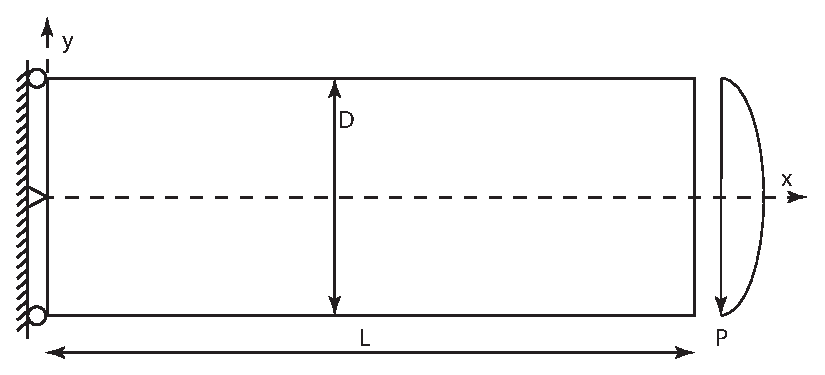
\includegraphics{isogeometric_sbfem/images/cantilever_beam_geo_bc.eps}}
        \caption{ Cantilever beam: Geometry and boundary conditions.}
        \label{iso_fig:cantilever_beam_geo_bc}
    \end{figure}
%
The geometry is: length $ L = \SI{8}{\meter} $, height $ D = \SI{4}{\meter} $.
The material properties are: Young’s modulus $ E = \SI{3e7}{\newton \per \square \meter}$ , Poisson’s ratio $ \nu = 0.25 $.
The parabolic shear force is $P = \SI{250}{\meter} $.
The exact solutions for the displacements are given by \citep{Aug2008}:
    \begin{equation}
        \begin{aligned}
            u(x,y) &= 
                \frac{Py}{6 \mean{E} I}
                \left[
                    \left(
                        6L-3x
                    \right)x
                    +\left(
                        2+ \mean{\nu}
                    \right)\left(
                        y^2-\frac{D^2}{4}
                    \right)
                \right]
            \\
            v(x,y) &=  
                -\frac{P}{6 \mean{E} I}
                \left[
                    3 \mean{\nu} y^2 \left(
                        L-x
                    \right)+
                    \left(
                        4+5 \mean{\nu}
                    \right)\frac{D^2x}{4}+
                    \left(
                        3L-x
                    \right)x^2
                \right]        
        \end{aligned}
    \label{iso_eq:cantilever_beam_displacement_solution}
    \end{equation}
%
where $I=D^3/12$ is the moment of inertia, $\mean{E}=E$, $\mean{\nu}=\nu$ and $\mean{E}=E/(1-\nu^2)$, $\mean{\nu}=\nu/(1-\nu)$ for plane stress and plane strain condition respectively.
The stress $\sigma$ can be expressed as \citep{Aug2008}
    \begin{subequations}
    \begin{align}
        \sigma_{xx} &= \frac{P(L-x)y}{I} \\
        \sigma_{yy} &= 0 \\
        \tau_{xy} &= -\frac{P}{2I} \left[
            \frac{D^2}{4} - y^2
        \right]
    \end{align}
    \label{iso_eq:cantilever_beam_stress_solution}
    \end{subequations}
%
The strain energy can be derived from Eq.~\ref{iso_eq:cantilever_beam_stress_solution} and Eq.~\ref{iso_eq:cantilever_beam_displacement_solution} as
\begin{equation}
\epsilon = 
    \frac{1}{2} \left(
        \frac{D^3 L^3 P^2}{36EI^2} + 
        \frac{D^5LP^2(1+v)}{60EI^2}
    \right)
    \label{iso_eq:cantilever_beam_energy_solution}
\end{equation}
\paragraph{}
In this example, rigid body motion is constrained by fixing 3 DOF on the left edge of the beam.
$u_x=0$ for points at $(0,-D/2)$ and $(0,D/2)$ and $u_y =0$ for point at $(0,0)$.
Surface tractions determined from the analytical solution of stress in Eq.~\ref{iso_eq:cantilever_beam_stress_solution} are applied on the boundary.

\paragraph{}
From the description in Section~\ref{iso_section:surface_traction}, the expression of the surface tractions must be transformed into NURBS-like representation before they can be applied.
The control points that describe a second order function as surface tractions in this example can be solved mathematically.
Assume the knot vector is evenly spaced and the shape functions is in second order, i.e. knot vector $K=[0,0,0,1,1,1]$.
Weight vector will be uniform because only the straight line is being interpolated, i.e. weight vector $w=[1,1,1]$.
Three basis functions used in B-Spline will be
    \begin{equation}
    \begin{aligned}
        N_1 & = (1-u)^2 \\
        N_2 & = 2u(1-u) \\
        N_3 & = u^2
    \end{aligned}
    \end{equation}
%
With the given targeted parabola as $y=ax^2+bx+c,x \in [0,1]$, the generalized control points for the NURBS curve will be
    \begin{equation}
        P= \begin{bmatrix}
            P_x \\
            P_y
        \end{bmatrix} = \begin{bmatrix}
            0 & m & 1 \\
            c & n & a+b+c
        \end{bmatrix}
    \end{equation}
%
where $m$ and $n$ are unknowns for the second control point.
B-spline curve $C=[N][P]$ then can be expressed as in parametric form as
    \begin{equation}
        \left\{
        \begin{aligned}
            x &= 2u(1-u)m + u^2 \\
            y &= c(1-u)^2 + 2u(1-u)n + (a+b+c)u^2
        \end{aligned}
        \right.
    \label{iso_eq:parabola_fitting_parametric}
    \end{equation}
%
After substituting Eq.~\ref{iso_eq:parabola_fitting_parametric} into $y=ax^2+bx+c$, we then have the system of equations as
    \begin{equation}
        \begin{bmatrix}
            0 \\
            0 \\
            2c - 2n +a +b \\
            2n - 2c \\
            c
        \end{bmatrix} = 
        \begin{bmatrix}
            4am^2-4am+a \\
            -8am^2 + 4am \\
            4am^2 -2bm +b \\
            2bm \\
            c
        \end{bmatrix}
    \end{equation}
%
$m$ and $n$ then can be solved as
    \begin{equation}
        \left\{
        \begin{aligned}
            m &= \frac{1}{2} \\
            n &= \frac{b+2c}{2}
        \end{aligned}
        \right.
    \end{equation}
%
\paragraph{}
The numerical convergence of the relative error in the displacement norm and the relative error in the energy norm are shown in Fig.~\ref{iso_fig:cantilever_beam_convergence} for various order of NURBS basis functions with refinement.
Fig.~\ref{iso_fig:cantilever_beam_convergence} also shows the error in the displacement norm when quadratic Lagrange shape functions are used along each edge within the scaled boundary formulation.
It can be observed that NURBS basis functions yield superior accuracy when compared to Lagrange basis functions of the same order.
It is seen that as the order of the shape functions is increased, the error decreases while the convergence rate increases.
\begin{figure}
    \begin{subfigure}[b]{1\linewidth}
        \centering
        \scalebox{0.7}{
            % This file was created by matlab2tikz v0.4.6 running on MATLAB 8.2.
% Copyright (c) 2008--2014, Nico Schlömer <nico.schloemer@gmail.com>
% All rights reserved.
% Minimal pgfplots version: 1.3
% 
% The latest updates can be retrieved from
%   http://www.mathworks.com/matlabcentral/fileexchange/22022-matlab2tikz
% where you can also make suggestions and rate matlab2tikz.
% 
\begin{tikzpicture}

\begin{axis}[%
width=4.52083333333333in,
height=3.5146875in,
scale only axis,
xmode=log,
xmin=10,
xmax=1000,
xminorticks=true,
xlabel={Total DOF},
ymode=log,
ymin=1e-05,
ymax=1,
yminorticks=true,
ylabel={Error},
title={l2l Displacement  Error},
legend style={draw=black,fill=white,legend cell align=left}
]
\addplot [color=blue,solid,mark=square,mark options={solid}]
  table[row sep=crcr]{
20	0.223473837	\\
40	0.0493	\\
80	0.011281049	\\
160	0.00266076	\\
};
\addlegendentry{1st order};

\addplot [color=black!50!green,solid,mark=o,mark options={solid}]
  table[row sep=crcr]{
20	0.067810872	\\
40	0.003190002	\\
80	0.000250473	\\
160	2.27e-05	\\
};
\addlegendentry{2nd order};

\addplot [color=red,solid,mark=+,mark options={solid}]
  table[row sep=crcr]{
20	0.0713	\\
40	0.00707	\\
80	0.000688	\\
160	8.85e-05	\\
};
\addlegendentry{LNGL 2nd order};

\end{axis}
\end{tikzpicture}%
        }
        \label{iso_fig:cantilever_beam_displacement_convergence}
        \caption{the relative error in displacement norm $(L^2)$}
    \end{subfigure}
    
    \begin{subfigure}[b]{1\linewidth}
        \centering
        \scalebox{0.7}{
            % This file was created by matlab2tikz v0.4.6 running on MATLAB 8.2.
% Copyright (c) 2008--2014, Nico Schlömer <nico.schloemer@gmail.com>
% All rights reserved.
% Minimal pgfplots version: 1.3
% 
% The latest updates can be retrieved from
%   http://www.mathworks.com/matlabcentral/fileexchange/22022-matlab2tikz
% where you can also make suggestions and rate matlab2tikz.
% 
\begin{tikzpicture}

\begin{axis}[%
width=4.52083333333333in,
height=3.5146875in,
scale only axis,
xmode=log,
xmin=10,
xmax=1000,
xminorticks=true,
xlabel={Total DOF},
ymode=log,
ymin=0.001,
ymax=1,
yminorticks=true,
ylabel={Error},
title={l2l Strain Energy  Error},
legend style={draw=black,fill=white,legend cell align=left}
]
\addplot [color=blue,solid,mark=square,mark options={solid}]
  table[row sep=crcr]{
20	0.701427116670007	\\
40	0.417133072292284	\\
80	0.228254244210267	\\
160	0.119582607431014	\\
};
\addlegendentry{1st order};

\addplot [color=black!50!green,solid,mark=o,mark options={solid}]
  table[row sep=crcr]{
20	0.180496573374677	\\
40	0.02575787258296	\\
80	0.0046690470119715	\\
160	0.0010295630140987	\\
};
\addlegendentry{2nd order};

\addplot [color=red,solid,mark=+,mark options={solid}]
  table[row sep=crcr]{
20	0.304275389	\\
40	0.065	\\
80	0.014502273	\\
160	0.003385053	\\
};
\addlegendentry{LNGL 2nd order};

\end{axis}
\end{tikzpicture}%
        }
        \label{iso_fig:cantilever_beam_energy_convergence}
        \caption{the relative error in the energy norm}
    \end{subfigure}
\caption{Bending of thick cantilever beam: Convergence results}
\label{iso_fig:cantilever_beam_convergence}
\end{figure}
%


\subsection{Infinite plate with a circular hole}
\paragraph{}
In this example, an infinite plate with a traction free hole under uniaxial tension $(\sigma = 1 N/m^2 )$
along x-axis (see Fig.~\ref{iso_fig:circular_hole_geo_bc}) is considered.

    \begin{figure}[h!]
        \centering
        \scalebox{0.5}{
            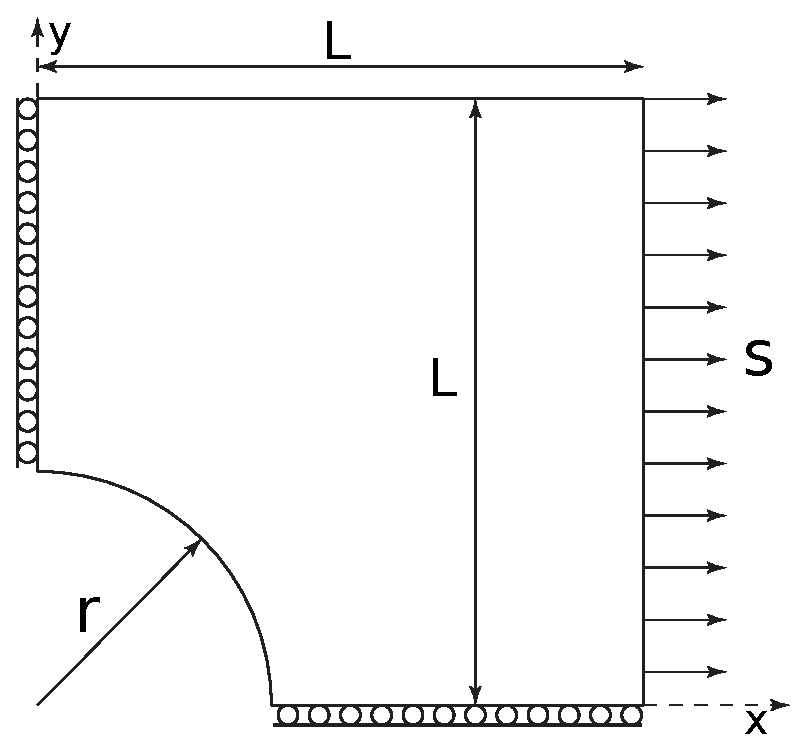
\includegraphics{isogeometric_sbfem/images/circular_hole_geo_bc.eps}
        }
        \caption{ Infinite plate with a circular hole: geometry and boundary conditions}
        \label{iso_fig:circular_hole_geo_bc}
    \end{figure}
%
The exact solution of the stresses in polar coordinate $(r,\theta)$ is given by \citep{Sukumar2001}:
    \begin{subequations}
        \begin{align}
            \sigma_{x}(r,\theta) &= 1 - \frac{a^2}{r^2} \left(
                \frac{3}{2} \cos2\theta +
                \cos4\theta
            \right) +
            \frac{3a^4}{2r^4} \cos4\theta\\
            \sigma_{y}(r,\theta) &= -\frac{a^2}{r^2} \left(
                \frac{1}{2} \cos2\theta -
                \cos4\theta
            \right) -
            \frac{3a^4}{2r^4} \cos4\theta\\
            \gamma_{xy}(r,\theta) &= -\frac{a^2}{r^2} \left(
                \frac{1}{2} \sin2\theta +
                \sin4\theta
            \right) -
            \frac{3a^4}{2r^4} \sin4\theta
        \end{align}
        \label{iso_eq:ex_chole_stress_sol}
    \end{subequations}
%
where $a$ is the radius of the hole.
Owing to symmetry, only one quarter of the plate is modeled.
% Fig. 10 shows a typical control net used for the study.
The material properties are: Young’s modulus $E = 100 N/m^2$ and Poisson’s ratio $\nu = 0.3$.
The closed form displacement in Cartesian coordinate is given as
    \begin{subequations}
        \begin{align}
            u_x(r,\theta) = \frac{R}{8G} \left[
                \frac{r}{R} (\kappa + 1) \cos\theta +
                2 \frac{R}{r} \left(
                    (1+ \kappa ) \cos\theta +
                    \cos3\theta
                \right) -
                2 \frac{R^3}{r^3}\cos3\theta
            \right] \\
            u_y(r,\theta) = \frac{R}{8G} \left[
                \frac{r}{R} (\kappa -3) \sin\theta +
                2 \frac{R}{r} \left(
                    (1 - \kappa) \sin\theta +
                    \sin3\theta
                \right) -
                2 \frac{R^3}{r^3}\sin3\theta
            \right]
        \end{align}
    \label{iso_eq:ex_chole_disp_sol}
    \end{subequations}
%
where $G$ is the shear modulus and $\kappa$ (Kolosov constant) is defined as
    \begin{equation}
        \kappa = \left\{
            \begin{aligned}   
                3-4 \nu \\
                \frac{3- \nu }{1+ \nu }    
            \end{aligned}
        \right.
    \label{iso_eq:kolosov_constant}
    \end{equation}
%
In this example, analytical tractions in Eq.~\ref{iso_eq:ex_chole_stress_sol} are applied on the boundary.
The left and bottom boundaries are constrained with a roller boundary condition. $u_x=0$ where $y=0$ and $u_y=0$ where $x=0$.

\paragraph{}
% result analysis
The convergence rate in terms of the displacement norm is shown in Fig.~\ref{iso_fig:circular_hole_convergence}
It is observed that the error decreases as the order of the shape functions is increased.
Another unique feature of the proposed method is that the method allows different type or order of shape functions to be employed for different segments of the boundary.
For example, in Fig.~\ref{iso_fig:circular_hole_mesh}, the arc A–B and the line segment B–C can be represented by different basis functions, i.e., the arc can be represented by NURBS and the line segment can be represented by conventional Lagrange basis functions.
Fig.~\ref{iso_fig:circular_hole_basis} shows the plot of the NURBS basis and Lagrange basis functions.
It can be seen that at point B, the shape function is continuous.
In order to assess the behavior, we represent the arc with quadratic NURBS and the straight lines with conventional Lagrange shape functions.
Since the NURBS are interpolatory at the ends, the compatibility requirement is automatically satisfied (see Fig.~\ref{iso_fig:circular_hole_shape_function_convergence}).
% The convergence of the relative error in the L 2 and H 1 is shown in Fig. 13.
The results from both the approaches converge with mesh refinement

    \begin{figure}
        \begin{subfigure}[b]{0.5\linewidth}
            \centering
            \scalebox{1}{
                % This file was created by matlab2tikz v0.4.6 running on MATLAB 8.0.
% Copyright (c) 2008--2014, Nico Schlömer <nico.schloemer@gmail.com>
% All rights reserved.
% Minimal pgfplots version: 1.3
% 
% The latest updates can be retrieved from
%   http://www.mathworks.com/matlabcentral/fileexchange/22022-matlab2tikz
% where you can also make suggestions and rate matlab2tikz.
% 
\begin{tikzpicture}[scale=0.6]

\begin{axis}[%
width=4.52083333333333in,
height=3.565625in,
scale only axis,
xmin=-0.197341513292434,
xmax=1.19734151329243,
ymin=-0.05,
ymax=1.05,
axis x line*=bottom,
axis y line*=left
]
\node[] at (-0.05,0.4) {$A$};
\node[] at (0.35,0) {$B$};
\addplot [color=blue,only marks,mark=o,mark options={solid},forget plot]
  table[row sep=crcr]{
0.6	0.6	\\
};
\label{archole_lab_sc}
\addplot [color=blue,dotted,mark size=4.2pt,mark=*,mark options={solid},forget plot]
  table[row sep=crcr]{
0.4	0	\\
0.4	0	\\
};
\label{archole_lab_cp}
\addplot [color=blue,dotted,mark size=4.2pt,mark=*,mark options={solid},forget plot]
  table[row sep=crcr]{
0.4	0	\\
0.7	0	\\
};
\addplot [color=blue,dotted,mark size=4.2pt,mark=*,mark options={solid},forget plot]
  table[row sep=crcr]{
0.7	0	\\
1	0	\\
};
\addplot [color=blue,dotted,mark size=4.2pt,mark=*,mark options={solid},forget plot]
  table[row sep=crcr]{
1	0	\\
1	0	\\
};
\addplot [color=blue,dotted,mark size=4.2pt,mark=*,mark options={solid},forget plot]
  table[row sep=crcr]{
1	0	\\
1	0.5	\\
};
\addplot [color=blue,dotted,mark size=4.2pt,mark=*,mark options={solid},forget plot]
  table[row sep=crcr]{
1	0.5	\\
1	1	\\
};
\addplot [color=blue,dotted,mark size=4.2pt,mark=*,mark options={solid},forget plot]
  table[row sep=crcr]{
1	1	\\
1	1	\\
};
\addplot [color=blue,dotted,mark size=4.2pt,mark=*,mark options={solid},forget plot]
  table[row sep=crcr]{
1	1	\\
0.5	1	\\
};
\addplot [color=blue,dotted,mark size=4.2pt,mark=*,mark options={solid},forget plot]
  table[row sep=crcr]{
0.5	1	\\
0	1	\\
};
\addplot [color=blue,dotted,mark size=4.2pt,mark=*,mark options={solid},forget plot]
  table[row sep=crcr]{
0	1	\\
0	1	\\
};
\addplot [color=blue,dotted,mark size=4.2pt,mark=*,mark options={solid},forget plot]
  table[row sep=crcr]{
0	1	\\
0	0.7	\\
};
\addplot [color=blue,dotted,mark size=4.2pt,mark=*,mark options={solid},forget plot]
  table[row sep=crcr]{
0	0.7	\\
0	0.4	\\
};
\addplot [color=blue,dotted,mark size=4.2pt,mark=*,mark options={solid},forget plot]
  table[row sep=crcr]{
0	0.4	\\
0	0.4	\\
};
\addplot [color=blue,dotted,mark size=4.2pt,mark=*,mark options={solid},forget plot]
  table[row sep=crcr]{
0	0.4	\\
0.4	0.4	\\
};
\addplot [color=blue,dotted,mark size=4.2pt,mark=*,mark options={solid},forget plot]
  table[row sep=crcr]{
0.4	0.4	\\
0.4	0	\\
};
\label{archole_lab_cpoly}
\addplot [color=blue,solid,forget plot]
  table[row sep=crcr]{
0	0.4	\\
0	1	\\
};
\label{archole_lab_mesh}
\addplot [color=blue,solid,forget plot]
  table[row sep=crcr]{
0	1	\\
1	1	\\
};
\addplot [color=blue,solid,forget plot]
  table[row sep=crcr]{
1	1	\\
1	0	\\
};
\addplot [color=blue,solid,forget plot]
  table[row sep=crcr]{
1	0	\\
0.4	0	\\
};
\addplot [color=blue,solid,forget plot]
  table[row sep=crcr]{
0.4	0	\\
0.399987538757663	0.00315734676388531	\\
0.399950155807063	0.00631449680545479	\\
0.399887853477391	0.0094712534146496	\\
0.39980063565047	0.0126274199059242	\\
0.39968850776051	0.0157827996305011	\\
0.399551476793777	0.0189371959886232	\\
0.399389551288152	0.0220904124418033	\\
0.399202741332597	0.0252422525250695	\\
0.398991058566535	0.0283925198592064	\\
0.398754516179117	0.0315410181629906	\\
0.398493128908403	0.0346875512654203	\\
0.398206913040442	0.037831923117938	\\
0.397895886408263	0.0409739378066453	\\
0.397560068390755	0.04411339956451	\\
0.397199479911468	0.0472501127835632	\\
0.396814143437303	0.050383882027087	\\
0.396404082977117	0.0535145120417917	\\
0.395969324080223	0.0566418077699807	\\
0.395509893834801	0.0597655743617044	\\
0.39502582086621	0.0628856171869003	\\
0.394517135335201	0.0660017418475197	\\
0.393983868936044	0.0691137541896398	\\
0.393426054894548	0.0722214603155609	\\
0.392843727965992	0.0753246665958872	\\
0.392236924432962	0.0784231796815912	\\
0.391605682103086	0.0815168065160609	\\
0.390950040306683	0.0846053543471276	\\
0.390270039894309	0.0876886307390765	\\
0.389565723234215	0.0907664435846361	\\
0.388837134209703	0.0938386011169475	\\
0.388084318216395	0.0969049119215133	\\
0.387307322159403	0.0999651849481233	\\
0.386506194450409	0.103019229522759	\\
0.385680985004645	0.106066855359471	\\
0.384831745237785	0.109107872572241	\\
0.383958528062743	0.112142091686806	\\
0.383061387886372	0.115169323652467	\\
0.382140380606078	0.118189379853868	\\
0.381195563606336	0.121202072122749	\\
0.380226995755113	0.124207212749668	\\
0.379234737400204	0.127204614495695	\\
0.378218850365467	0.130194090604085	\\
0.377179397946975	0.133175454811904	\\
0.37611644490907	0.136148521361645	\\
0.37503005748033	0.139113105012793	\\
0.373920303349439	0.142069021053371	\\
0.372787251660974	0.14501608531145	\\
0.371630973011092	0.147954114166619	\\
0.370451539443136	0.15088292456143	\\
0.369249024443144	0.153802334012804	\\
0.36802350293527	0.156712160623397	\\
0.366775051277116	0.159612223092936	\\
0.365503747254975	0.162502340729516	\\
0.364209670078985	0.165382333460854	\\
0.362892900378193	0.168252021845514	\\
0.361553520195529	0.171111227084084	\\
0.360191612982701	0.173959771030317	\\
0.358807263594985	0.176797476202232	\\
0.35740055828595	0.179624165793168	\\
0.355971584702072	0.182439663682806	\\
0.354520431877283	0.185243794448139	\\
0.353047190227419	0.188036383374401	\\
0.351551951544584	0.190817256465956	\\
0.350034808991438	0.193586240457136	\\
0.348495857095384	0.196343162823037	\\
0.346935191742686	0.199087851790273	\\
0.345352910172489	0.201820136347671	\\
0.343749110970765	0.204539846256931	\\
0.342123894064165	0.207246812063231	\\
0.340477360713798	0.209940865105787	\\
0.33880961350892	0.212621837528361	\\
0.33712075636054	0.215289562289715	\\
0.335410894494951	0.217943873174028	\\
0.333680134447167	0.220584604801243	\\
0.33192858405429	0.223211592637376	\\
0.33015635244879	0.225824673004767	\\
0.328363550051705	0.228423683092278	\\
0.32655028856576	0.231008460965435	\\
0.324716680968408	0.233578845576523	\\
0.322862841504794	0.236134676774611	\\
0.320988885680631	0.238675795315542	\\
0.319094930255008	0.241202042871846	\\
0.317181093233111	0.243713262042607	\\
0.315247493858877	0.246209296363272	\\
0.313294252607556	0.248689990315398	\\
0.311321491178212	0.251155189336343	\\
0.309329332486136	0.253604739828895	\\
0.307317900655188	0.256038489170843	\\
0.305287321010067	0.258456285724484	\\
0.303237720068498	0.260857978846075	\\
0.301169225533351	0.263243418895215	\\
0.299081966284684	0.265612457244172	\\
0.296976072371713	0.267964946287142	\\
0.294851675004712	0.270300739449443	\\
0.292708906546831	0.272619691196654	\\
0.290547900505856	0.274921657043674	\\
0.288368791525887	0.277206493563733	\\
0.286171715378949	0.279474058397323	\\
0.283956808956533	0.281724210261069	\\
0.281724210261069	0.283956808956533	\\
0.279474058397323	0.286171715378949	\\
0.277206493563733	0.288368791525887	\\
0.274921657043674	0.290547900505856	\\
0.272619691196654	0.292708906546831	\\
0.270300739449443	0.294851675004712	\\
0.267964946287142	0.296976072371713	\\
0.265612457244173	0.299081966284684	\\
0.263243418895215	0.301169225533351	\\
0.260857978846075	0.303237720068498	\\
0.258456285724484	0.305287321010067	\\
0.256038489170843	0.307317900655188	\\
0.253604739828895	0.309329332486136	\\
0.251155189336343	0.311321491178212	\\
0.248689990315398	0.313294252607556	\\
0.246209296363272	0.315247493858877	\\
0.243713262042607	0.317181093233111	\\
0.241202042871846	0.319094930255008	\\
0.238675795315542	0.320988885680631	\\
0.236134676774611	0.322862841504794	\\
0.233578845576523	0.324716680968408	\\
0.231008460965435	0.32655028856576	\\
0.228423683092278	0.328363550051705	\\
0.225824673004767	0.33015635244879	\\
0.223211592637376	0.33192858405429	\\
0.220584604801243	0.333680134447167	\\
0.217943873174028	0.335410894494951	\\
0.215289562289715	0.33712075636054	\\
0.212621837528361	0.33880961350892	\\
0.209940865105787	0.340477360713798	\\
0.207246812063231	0.342123894064165	\\
0.204539846256931	0.343749110970765	\\
0.201820136347671	0.345352910172489	\\
0.199087851790273	0.346935191742686	\\
0.196343162823038	0.348495857095384	\\
0.193586240457136	0.350034808991437	\\
0.190817256465956	0.351551951544584	\\
0.188036383374401	0.353047190227419	\\
0.185243794448139	0.354520431877283	\\
0.182439663682806	0.355971584702072	\\
0.179624165793168	0.35740055828595	\\
0.176797476202232	0.358807263594985	\\
0.173959771030317	0.360191612982701	\\
0.171111227084084	0.361553520195529	\\
0.168252021845514	0.362892900378193	\\
0.165382333460854	0.364209670078985	\\
0.162502340729516	0.365503747254975	\\
0.159612223092936	0.366775051277116	\\
0.156712160623397	0.36802350293527	\\
0.153802334012804	0.369249024443144	\\
0.15088292456143	0.370451539443136	\\
0.147954114166619	0.371630973011092	\\
0.14501608531145	0.372787251660974	\\
0.142069021053371	0.373920303349439	\\
0.139113105012793	0.37503005748033	\\
0.136148521361645	0.37611644490907	\\
0.133175454811905	0.377179397946975	\\
0.130194090604085	0.378218850365467	\\
0.127204614495695	0.379234737400204	\\
0.124207212749668	0.380226995755113	\\
0.121202072122749	0.381195563606336	\\
0.118189379853868	0.382140380606078	\\
0.115169323652467	0.383061387886372	\\
0.112142091686806	0.383958528062743	\\
0.109107872572241	0.384831745237785	\\
0.106066855359472	0.385680985004645	\\
0.103019229522759	0.386506194450409	\\
0.0999651849481234	0.387307322159403	\\
0.0969049119215133	0.388084318216395	\\
0.0938386011169475	0.388837134209703	\\
0.0907664435846361	0.389565723234215	\\
0.0876886307390766	0.390270039894309	\\
0.0846053543471276	0.390950040306683	\\
0.0815168065160609	0.391605682103086	\\
0.0784231796815913	0.392236924432962	\\
0.0753246665958872	0.392843727965992	\\
0.0722214603155609	0.393426054894548	\\
0.0691137541896398	0.393983868936044	\\
0.0660017418475197	0.394517135335201	\\
0.0628856171869003	0.39502582086621	\\
0.0597655743617044	0.395509893834801	\\
0.0566418077699807	0.395969324080223	\\
0.0535145120417917	0.396404082977117	\\
0.0503838820270871	0.396814143437303	\\
0.0472501127835632	0.397199479911468	\\
0.0441133995645101	0.397560068390755	\\
0.0409739378066454	0.397895886408263	\\
0.037831923117938	0.398206913040442	\\
0.0346875512654203	0.398493128908403	\\
0.0315410181629906	0.398754516179117	\\
0.0283925198592064	0.398991058566535	\\
0.0252422525250695	0.399202741332597	\\
0.0220904124418033	0.399389551288152	\\
0.0189371959886233	0.399551476793777	\\
0.0157827996305011	0.39968850776051	\\
0.0126274199059243	0.39980063565047	\\
0.00947125341464964	0.399887853477391	\\
0.00631449680545488	0.399950155807063	\\
0.00315734676388529	0.399987538757663	\\
2.44929359829471e-17	0.4	\\
};
\end{axis}
\end{tikzpicture}%
            }            
        \end{subfigure}
        \begin{subfigure}[b]{0.5\linewidth}
            \centering
            \scalebox{1}{
                % This file was created by matlab2tikz v0.4.6 running on MATLAB 8.0.
% Copyright (c) 2008--2014, Nico Schlömer <nico.schloemer@gmail.com>
% All rights reserved.
% Minimal pgfplots version: 1.3
% 
% The latest updates can be retrieved from
%   http://www.mathworks.com/matlabcentral/fileexchange/22022-matlab2tikz
% where you can also make suggestions and rate matlab2tikz.
% 
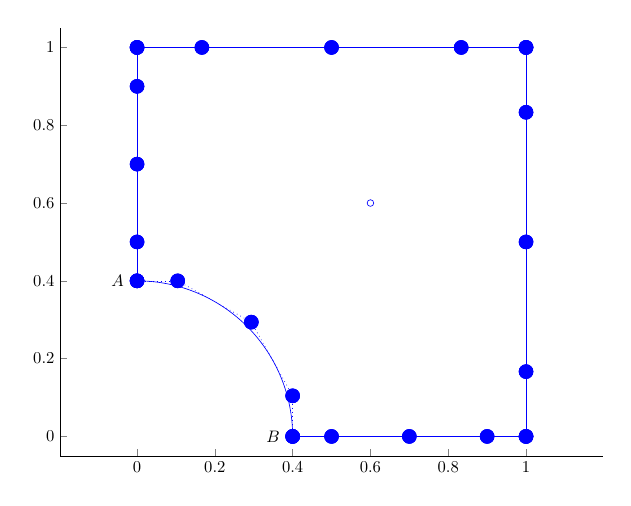
\begin{tikzpicture}[scale=0.6]

\begin{axis}[%
width=4.52083333333333in,
height=3.565625in,
scale only axis,
xmin=-0.197341513292434,
xmax=1.19734151329243,
ymin=-0.05,
ymax=1.05,
axis x line*=bottom,
axis y line*=left
]
\node[] at (-0.05,0.4) {$A$};
\node[] at (0.35,0) {$B$};
\addplot [color=blue,only marks,mark=o,mark options={solid},forget plot]
  table[row sep=crcr]{
0.6	0.6	\\
};
\addplot [color=blue,dotted,mark size=4.2pt,mark=*,mark options={solid},forget plot]
  table[row sep=crcr]{
0.4	0	\\
0.4	0	\\
};
\addplot [color=blue,dotted,mark size=4.2pt,mark=*,mark options={solid},forget plot]
  table[row sep=crcr]{
0.4	0	\\
0.5	0	\\
};
\addplot [color=blue,dotted,mark size=4.2pt,mark=*,mark options={solid},forget plot]
  table[row sep=crcr]{
0.5	0	\\
0.7	0	\\
};
\addplot [color=blue,dotted,mark size=4.2pt,mark=*,mark options={solid},forget plot]
  table[row sep=crcr]{
0.7	0	\\
0.9	1.11022302462516e-16	\\
};
\addplot [color=blue,dotted,mark size=4.2pt,mark=*,mark options={solid},forget plot]
  table[row sep=crcr]{
0.9	1.11022302462516e-16	\\
1	0	\\
};
\addplot [color=blue,dotted,mark size=4.2pt,mark=*,mark options={solid},forget plot]
  table[row sep=crcr]{
1	0	\\
1	0	\\
};
\addplot [color=blue,dotted,mark size=4.2pt,mark=*,mark options={solid},forget plot]
  table[row sep=crcr]{
1	0	\\
1	0.166666666666667	\\
};
\addplot [color=blue,dotted,mark size=4.2pt,mark=*,mark options={solid},forget plot]
  table[row sep=crcr]{
1	0.166666666666667	\\
1	0.5	\\
};
\addplot [color=blue,dotted,mark size=4.2pt,mark=*,mark options={solid},forget plot]
  table[row sep=crcr]{
1	0.5	\\
1	0.833333333333333	\\
};
\addplot [color=blue,dotted,mark size=4.2pt,mark=*,mark options={solid},forget plot]
  table[row sep=crcr]{
1	0.833333333333333	\\
1	1	\\
};
\addplot [color=blue,dotted,mark size=4.2pt,mark=*,mark options={solid},forget plot]
  table[row sep=crcr]{
1	1	\\
1	1	\\
};
\addplot [color=blue,dotted,mark size=4.2pt,mark=*,mark options={solid},forget plot]
  table[row sep=crcr]{
1	1	\\
0.833333333333333	1	\\
};
\addplot [color=blue,dotted,mark size=4.2pt,mark=*,mark options={solid},forget plot]
  table[row sep=crcr]{
0.833333333333333	1	\\
0.5	1	\\
};
\addplot [color=blue,dotted,mark size=4.2pt,mark=*,mark options={solid},forget plot]
  table[row sep=crcr]{
0.5	1	\\
0.166666666666667	1	\\
};
\addplot [color=blue,dotted,mark size=4.2pt,mark=*,mark options={solid},forget plot]
  table[row sep=crcr]{
0.166666666666667	1	\\
0	1	\\
};
\addplot [color=blue,dotted,mark size=4.2pt,mark=*,mark options={solid},forget plot]
  table[row sep=crcr]{
0	1	\\
0	1	\\
};
\addplot [color=blue,dotted,mark size=4.2pt,mark=*,mark options={solid},forget plot]
  table[row sep=crcr]{
0	1	\\
0	0.9	\\
};
\addplot [color=blue,dotted,mark size=4.2pt,mark=*,mark options={solid},forget plot]
  table[row sep=crcr]{
0	0.9	\\
0	0.7	\\
};
\addplot [color=blue,dotted,mark size=4.2pt,mark=*,mark options={solid},forget plot]
  table[row sep=crcr]{
0	0.7	\\
1.11022302462516e-16	0.5	\\
};
\addplot [color=blue,dotted,mark size=4.2pt,mark=*,mark options={solid},forget plot]
  table[row sep=crcr]{
1.11022302462516e-16	0.5	\\
0	0.4	\\
};
\addplot [color=blue,dotted,mark size=4.2pt,mark=*,mark options={solid},forget plot]
  table[row sep=crcr]{
0	0.4	\\
0	0.4	\\
};
\addplot [color=blue,dotted,mark size=4.2pt,mark=*,mark options={solid},forget plot]
  table[row sep=crcr]{
0	0.4	\\
0.104481549985497	0.4	\\
};
\addplot [color=blue,dotted,mark size=4.2pt,mark=*,mark options={solid},forget plot]
  table[row sep=crcr]{
0.104481549985497	0.4	\\
0.293836321356054	0.293836321356054	\\
};
\addplot [color=blue,dotted,mark size=4.2pt,mark=*,mark options={solid},forget plot]
  table[row sep=crcr]{
0.293836321356054	0.293836321356054	\\
0.4	0.104481549985497	\\
};
\addplot [color=blue,dotted,mark size=4.2pt,mark=*,mark options={solid},forget plot]
  table[row sep=crcr]{
0.4	0.104481549985497	\\
0.4	0	\\
};
\addplot [color=blue,solid,forget plot]
  table[row sep=crcr]{
0	0.4	\\
0	1	\\
};
\addplot [color=blue,solid,forget plot]
  table[row sep=crcr]{
0	1	\\
1	1	\\
};
\addplot [color=blue,solid,forget plot]
  table[row sep=crcr]{
1	1	\\
1	0	\\
};
\addplot [color=blue,solid,forget plot]
  table[row sep=crcr]{
1	0	\\
0.4	0	\\
};
\addplot [color=blue,solid,forget plot]
  table[row sep=crcr]{
0.4	0	\\
0.399987538757663	0.00315734676388531	\\
0.399950155807063	0.00631449680545479	\\
0.399887853477391	0.0094712534146496	\\
0.39980063565047	0.0126274199059242	\\
0.39968850776051	0.0157827996305011	\\
0.399551476793777	0.0189371959886232	\\
0.399389551288152	0.0220904124418033	\\
0.399202741332597	0.0252422525250695	\\
0.398991058566535	0.0283925198592064	\\
0.398754516179117	0.0315410181629906	\\
0.398493128908403	0.0346875512654203	\\
0.398206913040442	0.037831923117938	\\
0.397895886408263	0.0409739378066453	\\
0.397560068390755	0.04411339956451	\\
0.397199479911468	0.0472501127835632	\\
0.396814143437303	0.050383882027087	\\
0.396404082977117	0.0535145120417917	\\
0.395969324080223	0.0566418077699807	\\
0.395509893834801	0.0597655743617044	\\
0.39502582086621	0.0628856171869003	\\
0.394517135335201	0.0660017418475197	\\
0.393983868936044	0.0691137541896398	\\
0.393426054894548	0.0722214603155609	\\
0.392843727965992	0.0753246665958872	\\
0.392236924432962	0.0784231796815912	\\
0.391605682103086	0.0815168065160609	\\
0.390950040306683	0.0846053543471276	\\
0.390270039894309	0.0876886307390765	\\
0.389565723234215	0.0907664435846361	\\
0.388837134209703	0.0938386011169475	\\
0.388084318216395	0.0969049119215133	\\
0.387307322159403	0.0999651849481233	\\
0.386506194450409	0.103019229522759	\\
0.385680985004645	0.106066855359471	\\
0.384831745237785	0.109107872572241	\\
0.383958528062743	0.112142091686806	\\
0.383061387886372	0.115169323652467	\\
0.382140380606078	0.118189379853868	\\
0.381195563606336	0.121202072122749	\\
0.380226995755113	0.124207212749668	\\
0.379234737400204	0.127204614495695	\\
0.378218850365467	0.130194090604085	\\
0.377179397946975	0.133175454811904	\\
0.37611644490907	0.136148521361645	\\
0.37503005748033	0.139113105012793	\\
0.373920303349439	0.142069021053371	\\
0.372787251660974	0.14501608531145	\\
0.371630973011092	0.147954114166619	\\
0.370451539443136	0.15088292456143	\\
0.369249024443144	0.153802334012804	\\
0.36802350293527	0.156712160623397	\\
0.366775051277116	0.159612223092936	\\
0.365503747254975	0.162502340729516	\\
0.364209670078985	0.165382333460854	\\
0.362892900378193	0.168252021845514	\\
0.361553520195529	0.171111227084084	\\
0.360191612982701	0.173959771030317	\\
0.358807263594985	0.176797476202232	\\
0.35740055828595	0.179624165793168	\\
0.355971584702072	0.182439663682806	\\
0.354520431877283	0.185243794448139	\\
0.353047190227419	0.188036383374401	\\
0.351551951544584	0.190817256465956	\\
0.350034808991438	0.193586240457136	\\
0.348495857095384	0.196343162823037	\\
0.346935191742686	0.199087851790273	\\
0.345352910172489	0.201820136347671	\\
0.343749110970765	0.204539846256931	\\
0.342123894064165	0.207246812063231	\\
0.340477360713798	0.209940865105787	\\
0.33880961350892	0.212621837528361	\\
0.33712075636054	0.215289562289715	\\
0.335410894494951	0.217943873174028	\\
0.333680134447167	0.220584604801243	\\
0.33192858405429	0.223211592637376	\\
0.33015635244879	0.225824673004767	\\
0.328363550051705	0.228423683092278	\\
0.32655028856576	0.231008460965435	\\
0.324716680968408	0.233578845576523	\\
0.322862841504794	0.236134676774611	\\
0.320988885680631	0.238675795315542	\\
0.319094930255008	0.241202042871846	\\
0.317181093233111	0.243713262042607	\\
0.315247493858877	0.246209296363272	\\
0.313294252607556	0.248689990315398	\\
0.311321491178212	0.251155189336343	\\
0.309329332486136	0.253604739828895	\\
0.307317900655188	0.256038489170843	\\
0.305287321010067	0.258456285724484	\\
0.303237720068498	0.260857978846075	\\
0.301169225533351	0.263243418895215	\\
0.299081966284684	0.265612457244172	\\
0.296976072371713	0.267964946287142	\\
0.294851675004712	0.270300739449443	\\
0.292708906546831	0.272619691196654	\\
0.290547900505856	0.274921657043674	\\
0.288368791525887	0.277206493563733	\\
0.286171715378949	0.279474058397323	\\
0.283956808956533	0.281724210261069	\\
0.281724210261069	0.283956808956533	\\
0.279474058397323	0.286171715378949	\\
0.277206493563733	0.288368791525887	\\
0.274921657043674	0.290547900505856	\\
0.272619691196654	0.292708906546831	\\
0.270300739449443	0.294851675004712	\\
0.267964946287142	0.296976072371713	\\
0.265612457244173	0.299081966284684	\\
0.263243418895215	0.301169225533351	\\
0.260857978846075	0.303237720068498	\\
0.258456285724484	0.305287321010067	\\
0.256038489170843	0.307317900655188	\\
0.253604739828895	0.309329332486136	\\
0.251155189336343	0.311321491178212	\\
0.248689990315398	0.313294252607556	\\
0.246209296363272	0.315247493858877	\\
0.243713262042607	0.317181093233111	\\
0.241202042871846	0.319094930255008	\\
0.238675795315542	0.320988885680631	\\
0.236134676774611	0.322862841504794	\\
0.233578845576523	0.324716680968408	\\
0.231008460965435	0.32655028856576	\\
0.228423683092278	0.328363550051705	\\
0.225824673004767	0.33015635244879	\\
0.223211592637376	0.33192858405429	\\
0.220584604801243	0.333680134447167	\\
0.217943873174028	0.335410894494951	\\
0.215289562289715	0.33712075636054	\\
0.212621837528361	0.33880961350892	\\
0.209940865105787	0.340477360713798	\\
0.207246812063231	0.342123894064165	\\
0.204539846256931	0.343749110970765	\\
0.201820136347671	0.345352910172489	\\
0.199087851790273	0.346935191742686	\\
0.196343162823038	0.348495857095384	\\
0.193586240457136	0.350034808991437	\\
0.190817256465956	0.351551951544584	\\
0.188036383374401	0.353047190227419	\\
0.185243794448139	0.354520431877283	\\
0.182439663682806	0.355971584702072	\\
0.179624165793168	0.35740055828595	\\
0.176797476202232	0.358807263594985	\\
0.173959771030317	0.360191612982701	\\
0.171111227084084	0.361553520195529	\\
0.168252021845514	0.362892900378193	\\
0.165382333460854	0.364209670078985	\\
0.162502340729516	0.365503747254975	\\
0.159612223092936	0.366775051277116	\\
0.156712160623397	0.36802350293527	\\
0.153802334012804	0.369249024443144	\\
0.15088292456143	0.370451539443136	\\
0.147954114166619	0.371630973011092	\\
0.14501608531145	0.372787251660974	\\
0.142069021053371	0.373920303349439	\\
0.139113105012793	0.37503005748033	\\
0.136148521361645	0.37611644490907	\\
0.133175454811905	0.377179397946975	\\
0.130194090604085	0.378218850365467	\\
0.127204614495695	0.379234737400204	\\
0.124207212749668	0.380226995755113	\\
0.121202072122749	0.381195563606336	\\
0.118189379853868	0.382140380606078	\\
0.115169323652467	0.383061387886372	\\
0.112142091686806	0.383958528062743	\\
0.109107872572241	0.384831745237785	\\
0.106066855359472	0.385680985004645	\\
0.103019229522759	0.386506194450409	\\
0.0999651849481234	0.387307322159403	\\
0.0969049119215133	0.388084318216395	\\
0.0938386011169475	0.388837134209703	\\
0.0907664435846361	0.389565723234215	\\
0.0876886307390766	0.390270039894309	\\
0.0846053543471276	0.390950040306683	\\
0.0815168065160609	0.391605682103086	\\
0.0784231796815913	0.392236924432962	\\
0.0753246665958872	0.392843727965992	\\
0.0722214603155609	0.393426054894548	\\
0.0691137541896398	0.393983868936044	\\
0.0660017418475197	0.394517135335201	\\
0.0628856171869003	0.39502582086621	\\
0.0597655743617044	0.395509893834801	\\
0.0566418077699807	0.395969324080223	\\
0.0535145120417917	0.396404082977117	\\
0.0503838820270871	0.396814143437303	\\
0.0472501127835632	0.397199479911468	\\
0.0441133995645101	0.397560068390755	\\
0.0409739378066454	0.397895886408263	\\
0.037831923117938	0.398206913040442	\\
0.0346875512654203	0.398493128908403	\\
0.0315410181629906	0.398754516179117	\\
0.0283925198592064	0.398991058566535	\\
0.0252422525250695	0.399202741332597	\\
0.0220904124418033	0.399389551288152	\\
0.0189371959886233	0.399551476793777	\\
0.0157827996305011	0.39968850776051	\\
0.0126274199059243	0.39980063565047	\\
0.00947125341464964	0.399887853477391	\\
0.00631449680545488	0.399950155807063	\\
0.00315734676388529	0.399987538757663	\\
2.44929359829471e-17	0.4	\\
};
\end{axis}
\end{tikzpicture}%
            }
        \end{subfigure}
        \caption[Plate with circular hole: mesh]{
            Plate with circular hole: control net for two different discretizations.
            Control points ( 
                \tikz\draw[blue,fill=blue] (0,0) circle (.7ex);
            ), Boundary lines (
                \tikz[baseline=-0.5ex]\draw[blue,thick] (0,0) -- (0.5,0);
            ), Control polygon (
                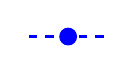
\begin{tikzpicture}[baseline=-0.5ex]
                    \draw[blue,thick,dashed] (0,0) -- (1,0);
                    \draw[blue,fill=blue] (0.5,0) circle (.7ex);
                \end{tikzpicture}
            ),
            Scaling center (
                \tikz[baseline=-0.5ex]\draw[blue] (0,0) circle (0.7ex);
            ).
        }
    \label{iso_fig:circular_hole_mesh}
    \end{figure}

    \begin{figure}
        \begin{subfigure}[b]{1\linewidth}
            \centering
            \scalebox{0.7}{
                % This file was created by matlab2tikz v0.4.6 running on MATLAB 8.2.
% Copyright (c) 2008--2014, Nico Schlömer <nico.schloemer@gmail.com>
% All rights reserved.
% Minimal pgfplots version: 1.3
% 
% The latest updates can be retrieved from
%   http://www.mathworks.com/matlabcentral/fileexchange/22022-matlab2tikz
% where you can also make suggestions and rate matlab2tikz.
% 
%
% defining custom colors
\definecolor{mycolor1}{rgb}{0.00000,0.75000,0.75000}%
\definecolor{mycolor2}{rgb}{0.75000,0.00000,0.75000}%
%
\begin{tikzpicture}

\begin{axis}[%
width=4.52083333333333in,
height=3.5146875in,
scale only axis,
xmode=log,
xmin=10,
xmax=1000,
xminorticks=true,
xlabel={Total DOF},
ymode=log,
ymin=1e-09,
ymax=0.1,
yminorticks=true,
ylabel={Error},
title={L2L Displacement Error},
legend style={draw=black,fill=white,legend cell align=left}
]
\addplot [color=blue,solid,mark=square,mark options={solid}]
  table[row sep=crcr]{
20	0.052647009	\\
40	0.015077369	\\
80	0.004598634	\\
160	0.001317239	\\
};
\addlegendentry{1st order};

\addplot [color=black!50!green,solid,mark=o,mark options={solid}]
  table[row sep=crcr]{
20	0.018330302	\\
40	0.000979438	\\
80	9.0447e-05	\\
160	7.10192e-06	\\
};
\addlegendentry{2nd order};

\addplot [color=red,solid,mark=triangle,mark options={solid,,rotate=180}]
  table[row sep=crcr]{
40	0.001028186	\\
80	6.4874e-06	\\
160	9.03877e-08	\\
};
\addlegendentry{4th order};

\addplot [color=mycolor1,solid,mark=asterisk,mark options={solid}]
  table[row sep=crcr]{
80	8.12048e-06	\\
160	7.13386e-09	\\
};
\addlegendentry{6th order};

\addplot [color=mycolor2,solid,mark=+,mark options={solid}]
  table[row sep=crcr]{
20	0.0371	\\
40	0.00228	\\
80	0.000316	\\
160	2.98e-05	\\
};
\addlegendentry{LNGL 2nd order};

\end{axis}
\end{tikzpicture}%
            }
            \label{iso_fig:circular_hole_displacement_convergence}
            \caption{the relative error in displacement norm $(L^2)$}
        \end{subfigure}
        
        \begin{subfigure}[b]{1\linewidth}
            \centering
            \scalebox{0.7}{
                % This file was created by matlab2tikz v0.4.6 running on MATLAB 8.2.
% Copyright (c) 2008--2014, Nico Schlömer <nico.schloemer@gmail.com>
% All rights reserved.
% Minimal pgfplots version: 1.3
% 
% The latest updates can be retrieved from
%   http://www.mathworks.com/matlabcentral/fileexchange/22022-matlab2tikz
% where you can also make suggestions and rate matlab2tikz.
% 
%
% defining custom colors
\definecolor{mycolor1}{rgb}{0.00000,0.75000,0.75000}%
\definecolor{mycolor2}{rgb}{0.75000,0.00000,0.75000}%
%
\begin{tikzpicture}

\begin{axis}[%
width=4.52083333333333in,
height=3.5146875in,
scale only axis,
xmode=log,
xmin=10,
xmax=1000,
xminorticks=true,
xlabel={Total DOF},
ymode=log,
ymin=1e-05,
ymax=1,
yminorticks=true,
ylabel={Error},
title={L2L Strain Energy Error},
legend style={draw=black,fill=white,legend cell align=left}
]
\addplot [color=blue,solid,mark=square,mark options={solid}]
  table[row sep=crcr]{
20	0.136951345	\\
40	0.070082184	\\
80	0.040238511	\\
160	0.02076975	\\
};
\addlegendentry{1st order};

\addplot [color=black!50!green,solid,mark=o,mark options={solid}]
  table[row sep=crcr]{
20	0.115220087	\\
40	0.0192672307117524	\\
80	0.002314805	\\
160	0.000499173	\\
};
\addlegendentry{2nd order};

\addplot [color=red,solid,mark=triangle,mark options={solid,,rotate=180}]
  table[row sep=crcr]{
40	0.028460196	\\
80	0.001326623	\\
160	6.43781e-05	\\
};
\addlegendentry{4th order};

\addplot [color=mycolor1,solid,mark=asterisk,mark options={solid}]
  table[row sep=crcr]{
80	0.000931962	\\
160	1.04862e-05	\\
};
\addlegendentry{6th order};

\addplot [color=mycolor2,solid,mark=+,mark options={solid}]
  table[row sep=crcr]{
20	0.196598384	\\
40	0.040130929	\\
80	0.00697	\\
160	0.00196	\\
};
\addlegendentry{LNGL 2nd order};

\end{axis}
\end{tikzpicture}%
            }
            \label{iso_fig:circular_hole_energy_convergence}
            \caption{the relative error in the energy norm}
        \end{subfigure}
    \caption{Bending of thick cantilever beam: Convergence results}
    \label{iso_fig:circular_hole_convergence}
    \end{figure}

    \begin{figure}
        \centering
        \scalebox{0.5}{
            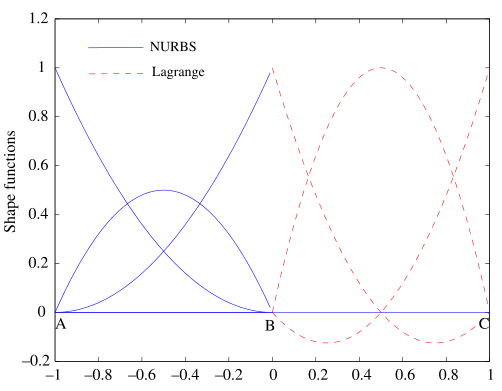
\includegraphics{isogeometric_sbfem/images/circular_hole_basis.png}
        }
        \caption{NURBS basis functions and Lagrange basis functions. It can be seen that at Point $B$, the shape functions are continuous}
        \label{iso_fig:circular_hole_basis}
    \end{figure}

    \begin{figure}
        \centering
        \scalebox{0.5}{
            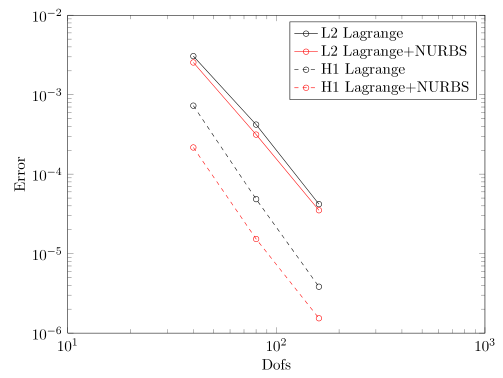
\includegraphics{isogeometric_sbfem/images/circular_hole_shape_function_convergence.png}
        }
        \caption{
            Infinite plate with a circular hole: Convergence results for the relative error in the displacement norm ($L^2$) and
                the relative error in the energy norm. In this case, the arc is represented with NURBS and Lagrange shape functions.
        }
        \label{iso_fig:circular_hole_shape_function_convergence}
    \end{figure}

\pagebreak

\subsection{L-shaped bracket}
\label{subsection:l_shaped_bracket}
\paragraph{}
In this example, an L-shaped bracket with isotropic material properties is considered.
Fig.~\ref{iso_fig:l_with_fillet_geo_bc} shows the geometry and the boundary conditions of the problem.
The L-shaped bracket is fixed at one end and subjected to downward vertical displacement at the other end.
Plain strain conditions are assumed.
    \begin{figure}[h!]
        \centering
        \scalebox{0.6}{
            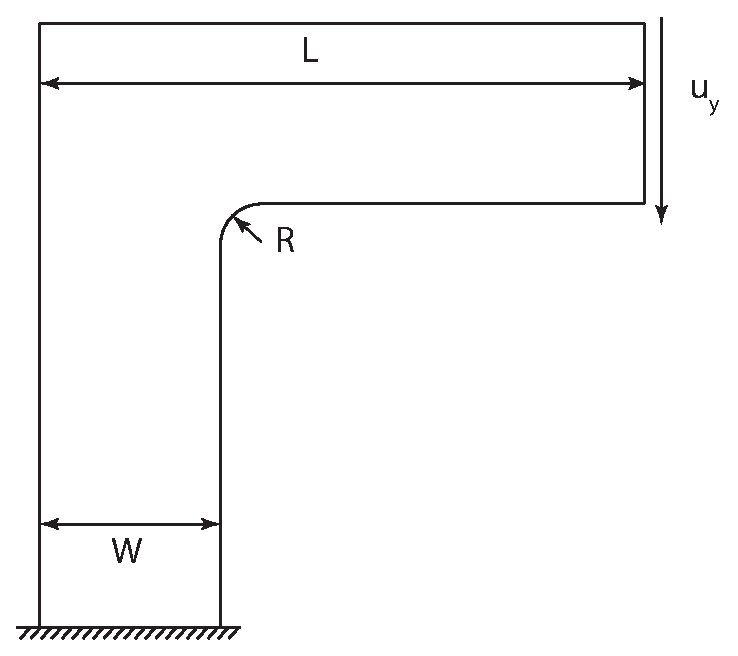
\includegraphics{isogeometric_sbfem/images/l_with_fillet_geo_bc.eps}
        }
        \caption{Geometry and boundary conditions} 
        \label{iso_fig:l_with_fillet_geo_bc}         
    \end{figure}
%
The dimension of the example is: $L=\SI{14}{\meter}$, $W=\SI{4}{\meter}$ and $R=\SI{1}{\meter}$.
While the material properties are: Young's modulus $E=\SI{1e3}{\mega\pascal}$ and poisson's ratio $\nu=0.3$.
This problem was studied in \citep{LIPTON2010357} by employing the conventional IGA.
In their study, the fillet was modeled as a separate path using biquadratic NURBS with nine control points.

\paragraph{}
In the present study, the control mesh is directly employed for the stress analysis.
However, as the domain does not meet the star convexity, we divide the domain into three subdomains (see Fig.~\ref{iso_fig:l_with_fillet_mesh}).
We employ NURBS to represent the fillet, whilst for the straight lines, we employ Lagrange basis functions.
The results from the present approach are compared with conventional finite element analysis using the commercial
    software ANSYS$^\circledR$.
    \begin{figure}[h!]
        \centering
        \scalebox{0.6}{
            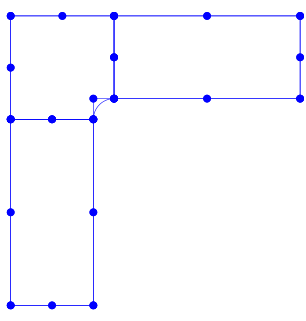
\includegraphics{isogeometric_sbfem/images/l_with_fillet_mesh.png}
        }
        \caption{Control net where `filled' circles represents control points}
        \label{iso_fig:l_with_fillet_mesh}
    \end{figure}
%
\paragraph{}
A total of $2000$ $8$-node quadrilateral elements were used for the finite element analysis.
Fig.~\ref{iso_fig:l_stress_contour} shows the von Mises equivalent stress for the L-shaped bracket with and without the fillet.
As expected, the no fillet case shows higher stress when compared to the L-shaped bracket with the fillet.
From Fig.~\ref{iso_fig:l_stress_contour}, it can be observed that the results from the present approach qualitatively match with the FE solution.
It should be noted that, the proposed method is computationally less intensive than the conventional IGA as it requires
    only the boundary information.
    \begin{figure}[h!]
        \begin{subfigure}[b]{0.5\linewidth}
            \centering
            \scalebox{0.5}{
                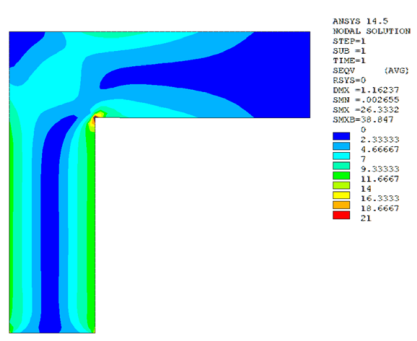
\includegraphics{isogeometric_sbfem/images/l_stress_contour_fem.png}
            }
            \caption{FEM}
        \end{subfigure}
        \begin{subfigure}[b]{0.5\linewidth}
            \centering
            \scalebox{0.5}{
                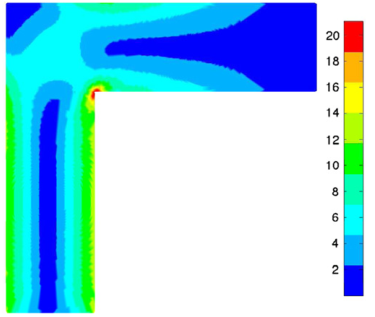
\includegraphics{isogeometric_sbfem/images/l_stress_contour_sbfem.png}
            }
            \caption{Isogeometric SBFEM}
        \end{subfigure}

        \begin{subfigure}[b]{0.5\linewidth}
            \centering
            \scalebox{0.5}{
                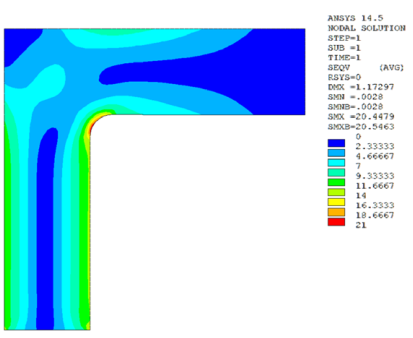
\includegraphics{isogeometric_sbfem/images/l_with_fillet_stress_contour_fem.png}
            }
            \caption{FEM}
        \end{subfigure}
        \begin{subfigure}[b]{0.5\linewidth}
            \centering
            \scalebox{0.5}{
                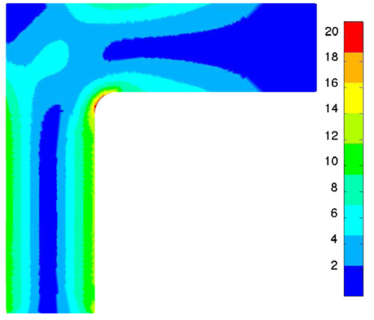
\includegraphics{isogeometric_sbfem/images/l_with_fillet_stress_contour_sbfem.png}
            }
            \caption{Isogeometric SBFEM}
        \end{subfigure}
        \caption[Von Mises equivalent stress contours for L-shaped bracket without and with fillet]{Von Mises equivalent stress contours for L-shaped bracket without and with fillet. The stress values are in Mpa}
        \label{iso_fig:l_stress_contour}
    \end{figure}
%

%=================================================================================================================================%
\paragraph{}
Next, we extend the present formulation to study the transient response of an L-shaped bracket.
The dimensions and the boundary conditions are shown in Fig.~\ref{iso_fig:l_dynamic_geo_bc}.
    \begin{figure}
        \begin{subfigure}[b]{1\linewidth}
            \centering
            \scalebox{0.8}{
                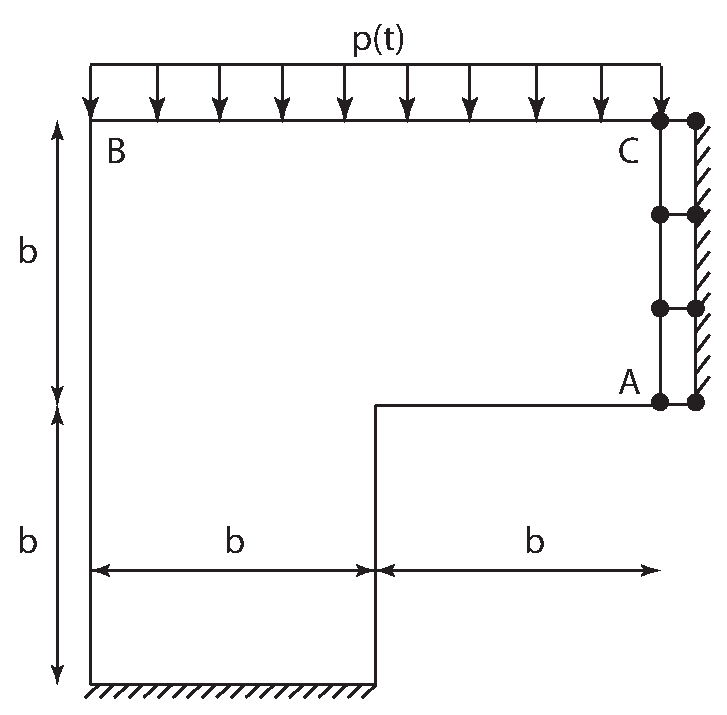
\includegraphics{isogeometric_sbfem/images/l_dynamic_geo_bc.eps}
            }
            \caption{without fillet}
        \end{subfigure}
        \begin{subfigure}[b]{1\linewidth}
            \centering
            \scalebox{0.8}{
                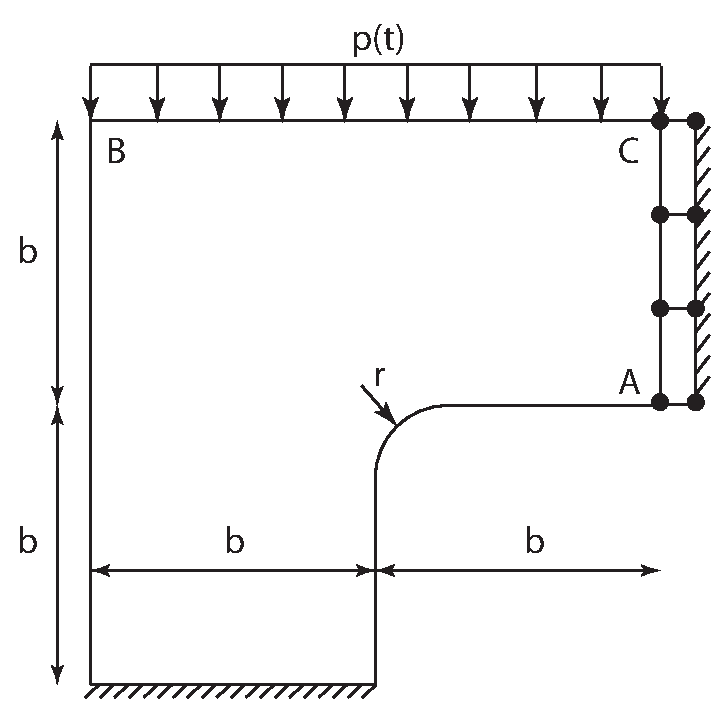
\includegraphics{isogeometric_sbfem/images/l_with_fillet_dynamic_geo_bc.eps}
            }
            \caption{without fillet}
        \end{subfigure}
        \caption{L-shaped bracket: geometry and boundary conditions for transient analysis}
        \label{iso_fig:l_dynamic_geo_bc}
    \end{figure}
%
\paragraph{}
In the example, $b=\SI{1}{\meter}$ and $r=\SI{0.2}{\meter}$.
A state of plane stress is considered and the material properties are:
    Young’s modulus $E = \SI{1}{\newton \per \square \meter}$ , poisson’s ratio, $\nu = 1/3$ and mass density, $\rho = \SI{1}{\kilo \gram \per \cubic \meter}$.
    The shear wave velocity is $c_s=\SI[parse-numbers = false]{\sqrt{3/8}}{\meter \per \second}$
    and the dilatational wave velocity $c_p=\SI[parse-numbers = false]{\sqrt{9/8}}{\meter \per \second}$
The order of the continued fraction used in Eq.~\ref{lr_eq:sbfem_dynamic_s_full} is chosen as $M_{cf} = 6$.
A uniform pressure $p(t)$ is applied at the side BC of the bracket.
The pressure varies as a triangular impulse in the time domain.
It reaches a peak value $p$ at time $t= 0.5b/c_p$ , reduces to $0$ at $t = b/c_p$ and stays at $0$ afterwards.
The time integration is carried out by using Newmark's method with $\gamma = 1/2$ and $\beta = 1/4$.
The time step is chosen as $\delta t = 0.025b/c_p$.

\paragraph{}
The calculation is performed for 3000 time steps.
For the Isogeometric-SBFEM, the arc is represented with quadratic NURBS functions and the straight lines are discretized with
    Lagrange basis functions.
As the problem domain does not satisfy the star convexity, the domain is sub-divided into three subdomains as done in the static example.
The scaling center for each of the subdomain is placed at the center of the subdomain.
To demonstrate the efficacy of the present formulation, the results are compared with those obtained using the conventional
    finite element method.
A FE mesh leading to a similar accuracy is identified from a convergence study.
The FE analysis is performed with the commercial software ANSYS$^\circledR$ (a total of 2000 8-node quadrilateral elements
    were employed for this study).

\paragraph{}
The vertical displacement responses at point A are plotted in Fig.~\ref{iso_fig:l_uy_dynamic_at_A} as a function of the dimensionless
    time $T = c_pt/b$.
It can be seen that the results from the present formulation agree well with the finite element solution.
    \begin{figure}
        \centering
        \scalebox{0.5}{
            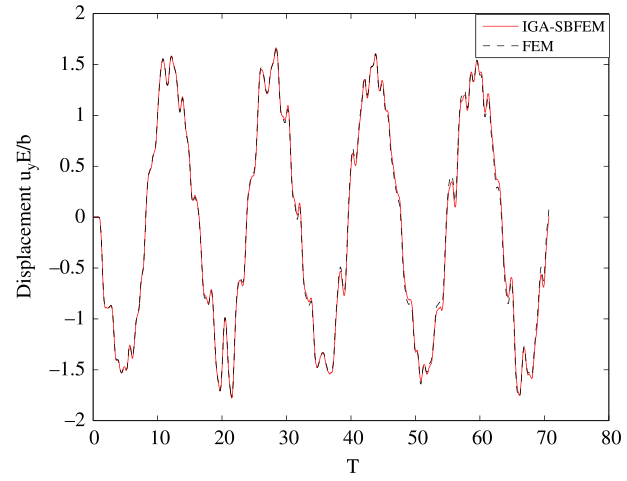
\includegraphics{isogeometric_sbfem/images/l_uy_at_A.png}
        }
    \caption{Vertical displacement of L-shaped bracket at Point A: comparison with conventional FE solution}
    \label{iso_fig:l_uy_dynamic_at_A}
    \end{figure}
%


\subsection{Circular disk with an edge crack in tension}

\paragraph{}
Next,we apply the present formulation to problems with strong discontinuities and singularities.
The unique feature of the proposed framework is that geometry is exactly represented by using NURBS and the singularities are captured semi-analytically without a priori knowledge of the asymptotic fields.
In the first example, consider a circular disk with an edge crack (see fig.~\ref{iso_fig:circular_disk_geo_bc}) with Young’s modulus $E=1N/m^2$ and Poisson's ratio $\nu=0.3$.
    \begin{figure}[h!]
        \centering
        \scalebox{0.4}{
            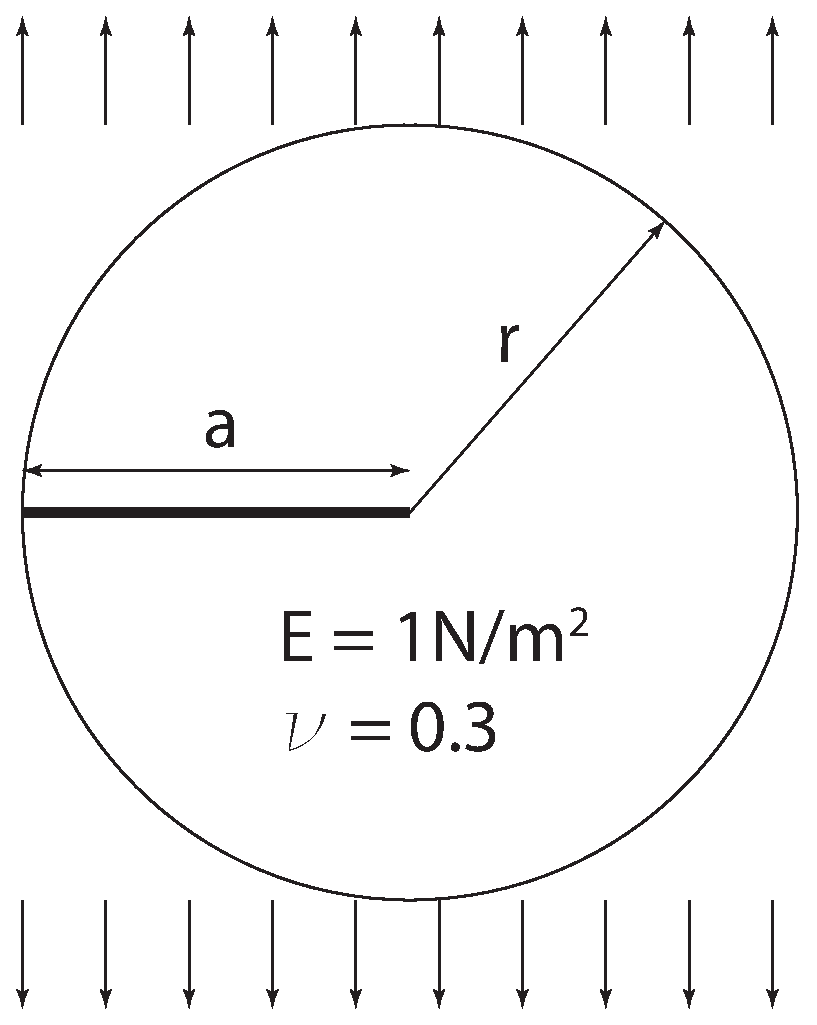
\includegraphics{isogeometric_sbfem/images/circular_disk_geo_bc.eps}
        }
        \caption{Circular disk with an edge crack}
        \label{iso_fig:circular_disk_geo_bc}
    \end{figure}

The analytical displacements solution for mode \RN{1} are given by:
    \begin{subequations}
        \begin{align}
            u_x &= \frac{1}{2}\left[
                \left(
                    \kappa + \frac{n}{2} + (-1)^n
                \right) \cos \left(
                    \frac{n\theta}{2}
                \right) -
                \frac{n}{2} \cos \left(
                    \left(
                        \frac{n}{2} -2
                    \right) \theta
                \right)
            \right]\\
            u_y &= \frac{1}{2}\left[
                \left(
                    \kappa - \frac{n}{2} - (-1)^n
                \right) \sin \left(
                    \frac{n\theta}{2}
                \right) +
                \frac{n}{2} \sin \left(
                    \left(
                        \frac{n}{2} -2
                    \right) \theta
                \right)
            \right]\\
        \end{align}
    \end{subequations}

where $\kappa$ is the Kolosov constant defined in eq.~\ref{iso_eq:kolosov_constant}.

The analytical stress solution for mode \RN{1} are given by:
    \begin{subequations}
        \begin{align}
            \sigma_{xx} &= \frac{n}{2}\left[
                \left(
                    2 + \frac{n}{2} + (-1)^n
                \right) \cos \left(
                    \left(
                        \frac{n}{2} - 1
                    \right)\theta
                \right) - \left(
                    \frac{n}{2} - 1
                \right)
                \cos \left(
                    \left(
                        \frac{n}{2} -3
                    \right) \theta
                \right)
            \right]\\
            \sigma_{yy} &= \frac{n}{2}\left[
                \left(
                    2 - \frac{n}{2} - (-1)^n
                \right) \cos \left(
                    \left(
                        \frac{n}{2} - 1
                    \right)\theta
                \right) + \left(
                    \frac{n}{2} - 1
                \right)
                \cos \left(
                    \left(
                        \frac{n}{2} -3
                    \right) \theta
                \right)
            \right]\\
            \tau_{xy} &= \frac{n}{2}\left[
                \left(
                    \frac{n}{2} - 1
                \right) \sin \left(
                    \left(
                        \frac{n}{2} - 3
                    \right)\theta
                \right) - \left(
                    \frac{n}{2} + (-1)^n
                \right)
                \sin \left(
                    \left(
                        \frac{n}{2} - 3
                    \right) \theta
                \right)
            \right]
        \end{align}
    \end{subequations}

\paragraph{}
In this example, the circular disk is represented by NURBS.
The control net and the location of control points are shown in fig.~\ref{iso_fig:circular_disk_mesh} for different NURBS order.
    \begin{figure}
        \begin{subfigure}[b]{0.5\linewidth}
            \centering
            \scalebox{0.4}{
                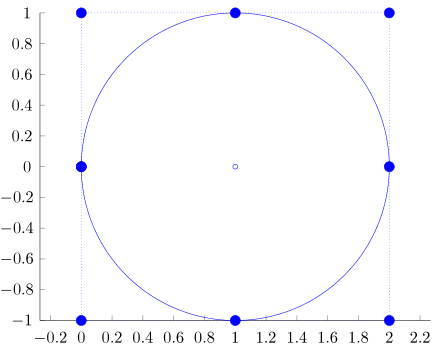
\includegraphics{isogeometric_sbfem/images/circular_disk_2nd_9cp.png}
            }
            \caption{9 control points, 2nd order}
        \end{subfigure}
        \begin{subfigure}[b]{0.5\linewidth}
            \centering
            \scalebox{0.4}{
                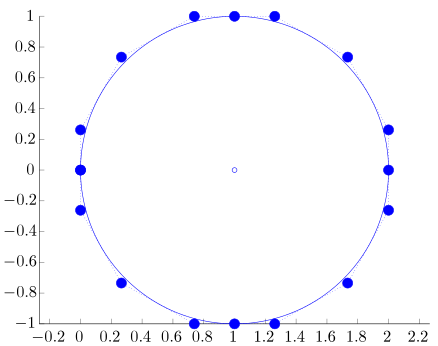
\includegraphics{isogeometric_sbfem/images/circular_disk_2nd_17cp.png}
            }
            \caption{9 control points, 2nd order}
        \end{subfigure}

        \begin{subfigure}[b]{0.5\linewidth}
            \centering
            \scalebox{0.4}{
                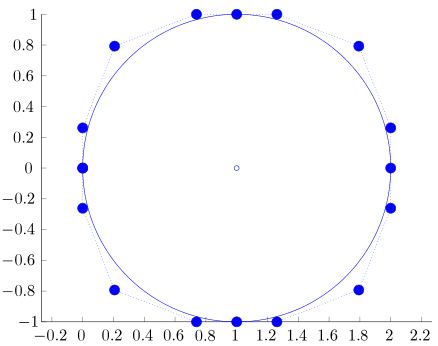
\includegraphics{isogeometric_sbfem/images/circular_disk_3rd_17cp.png}
            }
            \caption{9 control points, 2nd order}
        \end{subfigure}
        \begin{subfigure}[b]{0.5\linewidth}
            \centering
            \scalebox{0.4}{
                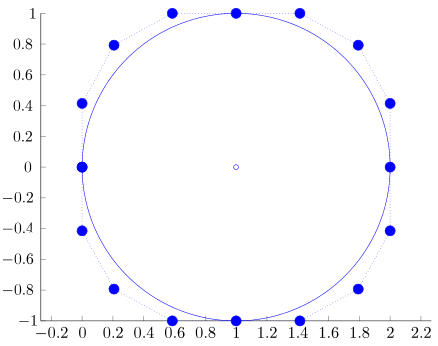
\includegraphics{isogeometric_sbfem/images/circular_disk_4th_17cp.png}
            }
            \caption{9 control points, 2nd order}
        \end{subfigure}
        \caption{Meshing of the circular disk with an edge notch}
        \label{iso_fig:circular_disk_mesh}
    \end{figure}

\paragraph{}
The circular disk is subjected to a far field tension and the displacement and the stress modes are computed by the proposed isogeometric SBFEM.
It is noted that only the boundary of the circular disk is discretized using the NURBS and no tensor product of the corresponding knot vectors is required to represent the unknown fields inside the domain.
The convergence of the numerical stress intensity factor (SIF) and the T-stress with mesh refinement is shown in Table 1.

\begin{table}[]
\caption{T-stress and stress intensity factors for circular disk with an edge crack.}
\label{iso_tab:circular_disk_res}
\begin{tabularx}{\textwidth}{XXXXXXX}
\toprule
    Total    &   \multicolumn{2}{c}{NURBS $p=2$} &\multicolumn{2}{c}{NURBS $p=4$} &\multicolumn{2}{c}{NURBS $p=6$}\\
    \cmidrule{2-7}
    DOF      &   SIF     &   T-stress            &SIF     &   T-stress            &SIF     &   T-stress           \\
    \cmidrule{1-1} \cmidrule{2-3} \cmidrule{4-5} \cmidrule{6-7}
    18       &   2.3520  &   2.9442              &        &                       &        &                      \\
    34       &   2.8693  &   5.1991              &2.8838  &5.4050                 &        &                      \\
    74       &   2.8838  &   5.3112              &2.8840  &5.3445                 &2.8840  &5.3447                \\
    130      &   2.8840  &   5.3318              &2.8840  &5.3444                 &2.8840  &5.3444                \\
\bottomrule
\end{tabularx}
\end{table}

\paragraph{}
It can be seen that with mesh refinement the SIF and the T-stress converge.
Increasing the order of the NURBS functions increases the convergence behavior.
Eq.~\ref{iso_eq:isosbfem_fracture_stress_field} is the parametric equation for the stress field in the polar coordinates $r$ and $\theta$.
The terms $\left(
        r_\eta^{\lambda_i+1}(\eta)
        \boldsymbol{\psi}_{\sigma_i}(\eta)
    \right)$
in eq.~\ref{iso_eq:isosbfem_fracture_stress_field} together with $\theta(\eta)$ in eq.~\ref{iso_eq:isosbfem_coordinate_transformation} are the stress modes describing the angular distribution at a constant radial coordinate $r$.
For the converged result, fig.~\ref{iso_fig:circular_disk_modes} shows the displacement and the stress distribution at a constant radial coordinate r around the crack tip for mode \RN{1} fracture.
Each of the stress modes is normalized with its value of $\sigma_{yy}=0^\circ$ .
    \begin{figure}[h!]
        \begin{subfigure}[b]{1\linewidth}
            \centering
            \scalebox{0.4}{
                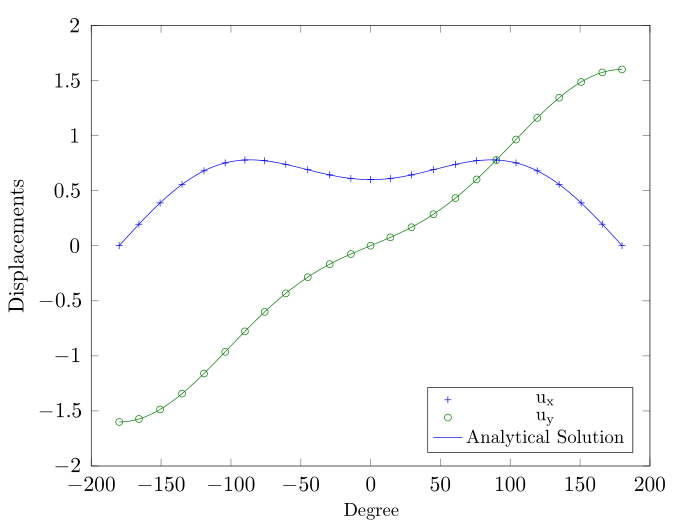
\includegraphics{isogeometric_sbfem/images/circular_disk_displacement_modes.png}
            }
            \caption{displacements}
        \end{subfigure}
        \begin{subfigure}[b]{1\linewidth}
            \centering
            \scalebox{0.4}{
                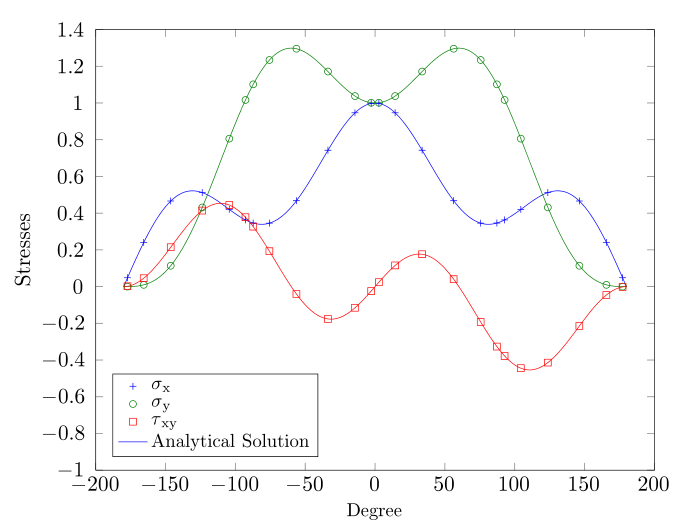
\includegraphics{isogeometric_sbfem/images/circular_disk_stress_modes.png}
            }
            \caption{stress}
        \end{subfigure}
    \caption{Displacement and stress modes of circular disk with an edge crack using cubic NURBS functions}
    \label{iso_fig:circular_disk_modes}
    \end{figure}

\paragraph{}
The results from the scaled boundary formulation are compared with the analytical solutions and a very good agreement is observed.
The convergence of the displacement and stress modes with h and p refinement is shown in fig.~\ref{iso_fig:circular_disk_convergence}.
It can be seen that with refinement the solution converges monotonically.
    \begin{figure}[h!]
        \begin{subfigure}[b]{1\linewidth}
            \centering
            \scalebox{0.65}{
                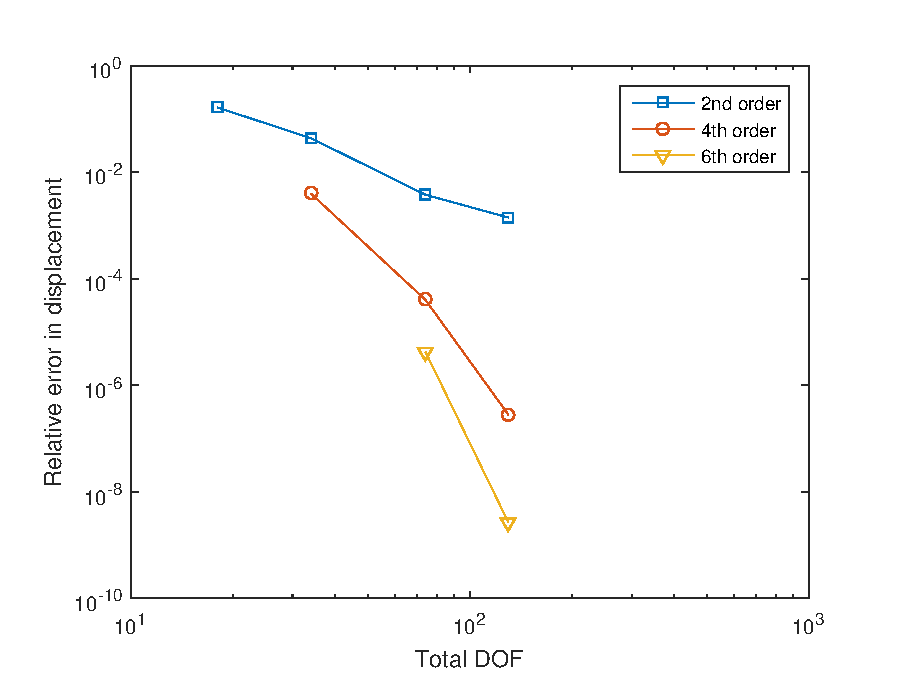
\includegraphics{isogeometric_sbfem/images/circular_disk_convergence_displacement.eps}
            }
            \caption{Displacement mode}
        \end{subfigure}

        \begin{subfigure}[b]{1\linewidth}
            \centering
            \scalebox{0.65}{
                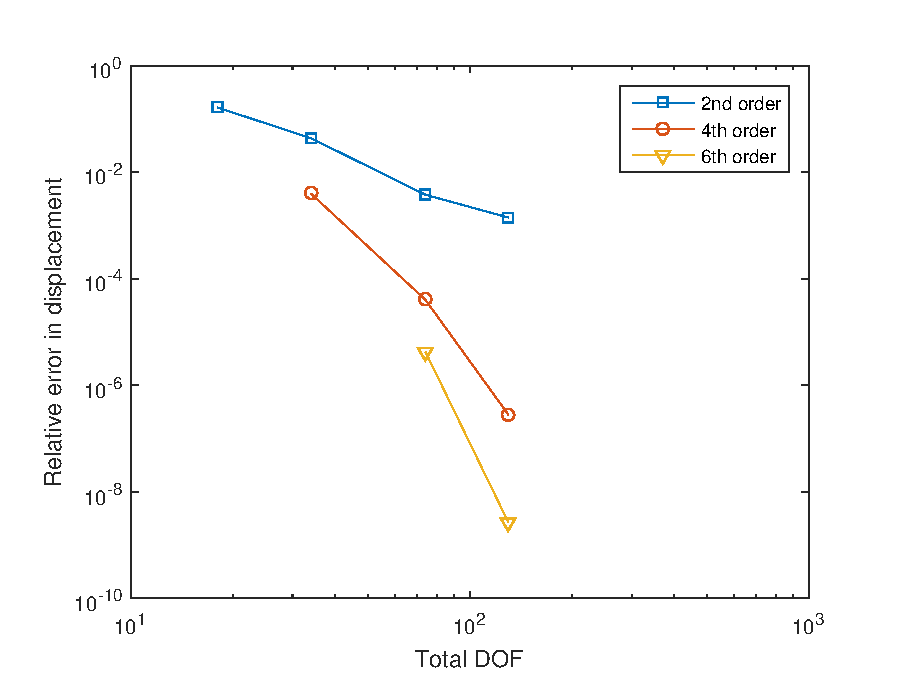
\includegraphics{isogeometric_sbfem/images/circular_disk_convergence_displacement.eps}
            }
            \caption{Displacement mode}
        \end{subfigure}
    \caption{Circular disk with an edge crack: convergence of the displacement mode and stress mode}
    \label{iso_fig:circular_disk_convergence}
    \end{figure}

\pagebreak

\subsection{Edge crack in tension}

\pagebreak

\subsection{Angled crack in an orthotropic body}

\paragraph{}
In this example, consider an orthotropic plate $(b/h = 1)$ with an angled center-crack of length $a/h = 0.5$ under uniform far field tension along the two opposite sides (see fig.~\ref{iso_fig:angled_crack_geo_bc}). 
    \begin{figure}
        \centering
        \scalebox{0.5}{
            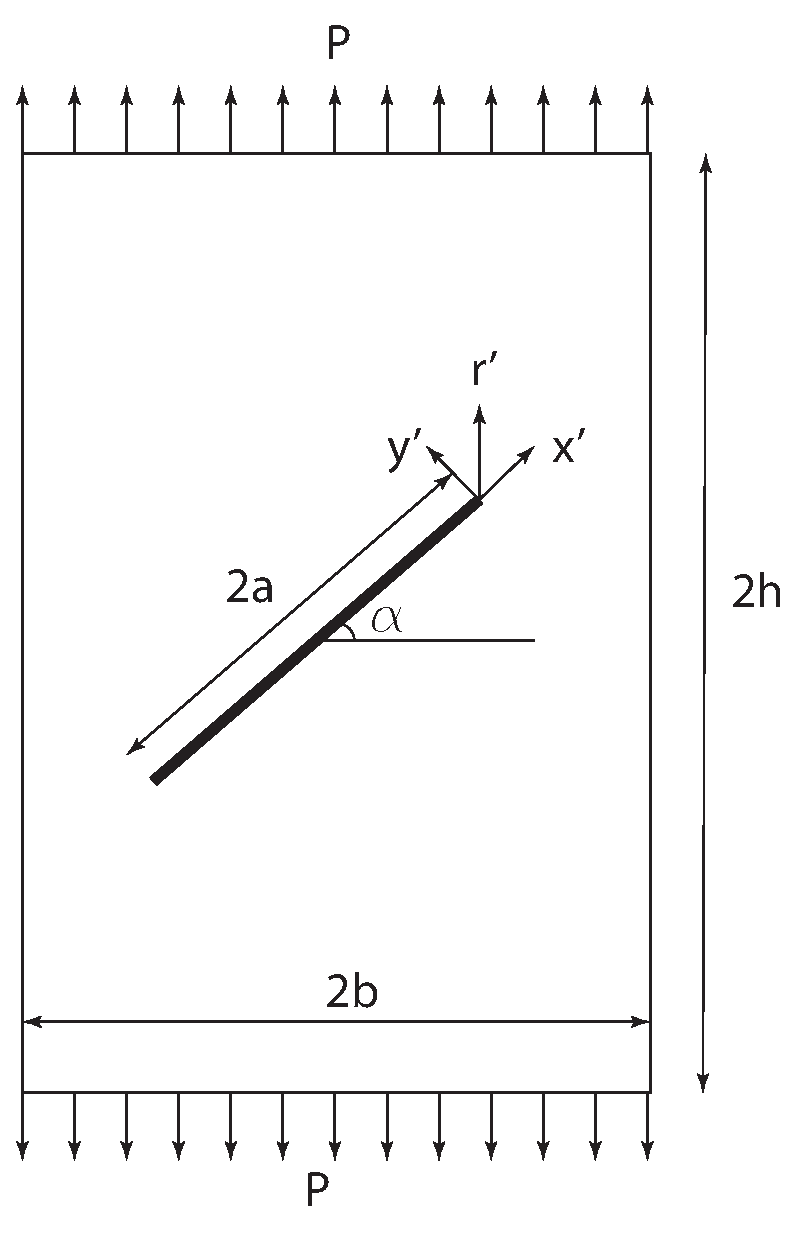
\includegraphics{isogeometric_sbfem/images/angled_crack_geo_bc.eps}
        }
        \caption{Angled crack in a rectangular orthotropic body: geometry}
        \label{iso_fig:angled_crack_geo_bc}
    \end{figure}

\paragraph{}
The elastic properties of the material are $E_{11} = E_{22}= E_{33}=15.4\times 10^6 psi$, $G_{12} = G_{23} = G_{13} = 15.7 \times 10^6 psi$, and $\nu_{12} = \nu_{23} = \nu_{13} = 0.4009$.
The results are compared with those obtained in \cite{Banks2005}.
The convergence of mode I and mode II SIF with mesh size is shown in tab.~\ref{iso_tab:angled_crack_convergence} for a crack at an angle $\alpha = \pi/12$.
The influence of the order of the shape functions is also shown.
It can be seen that increasing the number of degrees of freedom, the error in the numerical SIF decreases.
A very good agreement is observed.
\begin{table}
\caption{Convergence of the generalized stress intensity factors $
    (\mean{K_\RN{1}}, \mean{K_\RN{2}}) =
    (K_I,K_{II}) /
    P\sqrt(\pi a)
    $}
\label{iso_tab:angled_crack_convergence}
\begin{tabularx}{\textwidth}{XXXXX}
    \toprule
    \multirow{2}{*}{Order}& & \multicolumn{3}{c}{Number of DOF} \\
    \cmidrule{3-5}
    & & 160 & 240 & 320 \\
    \multirow{2}{*}{$2$}    &   $\mean{K_\RN{1}}$   &   1.2770  &   1.2723  &   1.2706  \\
                            &   $\mean{K_\RN{2}}$   &   0.2918  &   0.2915  &   0.2913  \\
    \multirow{2}{*}{$4$}    &   $\mean{K_\RN{1}}$   &   1.2700  &   1.2697  &   1.2697  \\
                            &   $\mean{K_\RN{2}}$   &   0.2914  &   0.2913  &   0.2913  \\
    \multirow{2}{*}{$6$}    &   $\mean{K_\RN{1}}$   &           &   1.2668  &   1.2670  \\
                            &   $\mean{K_\RN{2}}$   &           &   0.2913  &   0.2913  \\                           
    \midrule
    \bottomrule
\end{tabularx}
\end{table}

\paragraph{}
Also, increasing the order of the NURBS basis functions, the error decreases.
The influence of the crack orientation α on the mode \RN{1} and mode \RN{2} SIF is shown in tab.~\ref{iso_tab:angled_crack_sif_1} and tab.~\ref{iso_tab:angled_crack_sif_2}.
A total of 80 control points are used with different order of the NURBS basis functions.
It can be seen that a very good agreement is observed.
\begin{table}
\caption{Generalized stress intensity factors $K_\RN{1}/P\sqrt{\pi a}$ of angled crack in rectangular orthotropic body}
\label{iso_tab:angled_crack_sif_1}
\begin{tabularx}{\textwidth}{XXXXX}
    \toprule
    Angle   &   $K_\RN{1}$  &   \multicolumn{3}{c}{ }  \\
    \cmidrule{2-5} 
    $\alpha$&\cite{Banks2005}&  \multicolumn{3}{c}{Order of the curve}  \\
    \cmidrule{3-5} 
    & & 2 & 4 & 6 \\
    \midrule
    0         & 1.3755 & 1.3603 & 1.3583 & 1.3583 \\
    $\pi/12 $ & 1.2692 & 1.2706 & 1.2697 & 1.2670 \\
    $\pi/ 6 $ & 1.0268 & 1.0277 & 1.0270 & 1.0270 \\
    $\pi/ 4 $ & 0.6952 & 0.6941 & 0.6944 & 0.6943 \\
    $\pi /3 $ & 0.3579 & 0.3582 & 0.3580 & 0.3580 \\
    $5\pi/12$ & 0.1095 & 0.0996 & 0.1003 & 0.1004 \\
    \bottomrule
\end{tabularx}
\end{table}

\begin{table}
    \caption{Generalized stress intensity factors $K_\RN{2}/P\sqrt{\pi a}$ of angled crack in rectangular orthotropic body}
    \label{iso_tab:angled_crack_sif_2}
    \begin{tabularx}{\textwidth}{XXXXX}
        \toprule
        Angle   &   $K_\RN{2}$  &   \multicolumn{3}{c}{ }\\
        \cmidrule{2-5}
        $\alpha$&\cite{Banks2005}&  \multicolumn{3}{c}{Order of the curve}\\
        \cmidrule{3-5}
        & & 2 & 4 & 6 \\
        \midrule
        0         & 0.0000 & 0.0000 & 0.0000 & 0.0000 \\
        $\pi/12 $ & 0.2912 & 0.2914 & 0.2913 & 0.2913 \\
        $\pi/ 6 $ & 0.5092 & 0.5087 & 0.5093 & 0.5092 \\
        $\pi/ 4 $ & 0.5807 & 0.5948 & 0.5946 & 0.5946 \\
        $\pi /3 $ & 0.5248 & 0.5247 & 0.5248 & 0.5248 \\
        $5\pi/12$ & 0.3108 & 0.3119 & 0.3117 & 0.3117 \\
        \bottomrule
    \end{tabularx}
\end{table}

\pagebreak

\subsection{Transient analysis of bimaterial plate with a notch}

\pagebreak

%=================================================================================================================================%
\section{Conclusions}
\paragraph{}
In this chapter,the NURBS basis functions are employed to approximate the unknown fields in the circumferential direction within the framework of the SBFEM.
The accuracy, effectiveness and the convergence properties of the proposed method are demonstrated with benchmark problems in linear elasticity and linear elastic fracture mechanics.
From the numerical studies, it can be observed that the NURBS basis functions yield superior accuracy when compared to Lagrange basis functions of the same order.
The proposed method overcomes the disadvantages of both the isogeometric finite element analysis and the isogeometric boundary element method. 
Like in the IGAFEM no fundamental solution is required and like in the IGABEM the spatial dimension is reduced by one.
However, for complicated geometries, to meet the star convexity, subdivision into smaller sub-domains is required.
When applied to problems with singularities, the proposed method does not require additional functions to span the solution space.
Moreover, the proposed framework does not require internal discretization to study the dynamic response at high frequencies.
\pagebreak